%%%%%% Run at command line, run
%%%%%% xelatex grad-sample.tex 
%%%%%% for a few times to generate the output pdf file
\documentclass[12pt,oneside,openright,a4paper]{cpe-thai-project}

\usepackage[table,xcdraw]{xcolor}
\usepackage{polyglossia}
\setdefaultlanguage{thai}
\setotherlanguage{english}
\newfontfamily\thaifont[Script=Thai,Scale=1.23]{TH Sarabun New}


\defaultfontfeatures{Mapping=tex-text,Scale=1.23,LetterSpace=0.0}
\setmainfont[Scale=1.23,LetterSpace=0,WordSpace=1.0,FakeStretch=1.0]{TH Sarabun New}
%\setmathfont(Digits)[Scale=1.0,LetterSpace=0,FakeStretch=1.0]{Times New Roman}


%%%%%%%%%%%%%%%%%%%%%%%%%%%%%%%%%%%%%%%%%%%%%%%%%%%%%%%%%%%%%%%%%%%
% Customize below to suit your needs 
% The ones that are optional can be left blank. 
%%%%%%%%%%%%%%%%%%%%%%%%%%%%%%%%%%%%%%%%%%%%%%%%%%%%%%%%%%%%%%%%%%%
% First line of title
\def\disstitleone{Your Art Painter}   
% Second line of title
\def\disstitletwo{(จิตรกรผู้สร้างศิลปะของคุณ)}   
% Your first name and lastname
\def\dissauthor{Mr. Nawarit Longkhum}   % 1st member
%%% Put other group member names here ..
\def\dissauthortwo{Ms. Pataraphorn Tanutsiriteeradet​}   % 2nd member (optional)
\def\dissauthorthree{Ms. Sukasama   Chitakson}   % 3rd member (optional)


% The degree that you're persuing..
\def\dissdegree{Bachelor of Engineering} % Name of the degree
\def\dissdegreeabrev{B.Eng} % Abbreviation of the degree
\def\dissyear{2020}                   % Year of submission
\def\thaidissyear{2563}               % Year of submission (B.E.)

%%%%%%%%%%%%%%%%%%%%%%%%%%%%%%%%%%%%%%%%%%%%
% Your project and independent study committee..
%%%%%%%%%%%%%%%%%%%%%%%%%%%%%%%%%%%%%%%%%%%%
\def\dissadvisor{Dr.Nuttanart Facundes}  % Advisor
%%% Leave it empty if you have no Co-advisor
\def\disscoadvisor{}  % Co-advisor
\def\disscommitteetwo{Dr.Natasha Dejdumrong}  % 3rd committee member (optional)
\def\disscommitteethree{Dr.Unchalisa Taetragool}   % 4th committee member (optional) 
\def\disscommitteefour{Dr.Thumrongrat Amornraksa}    % 5th committee member (optional) 

\def\worktype{Project} %%  Project or Independent study
\def\disscredit{3}   %% 3 credits or 6 credits


\def\fieldofstudy{Computer Engineering} 
\def\department{Computer Engineering} 
\def\faculty{Engineering}

\def\thaifieldofstudy{วิศวกรรมคอมพิวเตอร์} 
\def\thaidepartment{วิศวกรรมคอมพิวเตอร์} 
\def\thaifaculty{วิศวกรรมศาสตร์}
 
\def\appendixnames{Appendix} %%% Appendices or Appendix

\def\thaiworktype{ปริญญานิพนธ์} %  Project or research project % 
\def\thaidisstitleone{จิตรกรผู้สร้างศิลปะของคุณ}
\def\thaidisstitletwo{Your Art Painter}
\def\thaidissauthor{นายนวฤทธิ์ หล่องคุ้ม}
\def\thaidissauthortwo{นางสาวภัทรพร ธนัชศิริธีรเดช} %Optional
\def\thaidissauthorthree{นางสาวสุกษมา จิตอักษร	} %Optional

\def\thaidissadvisor{ผศ.ดร.ณัฐนาถ 	ฟาคุนเด๊ซ}
%% Leave this empty if you have no co-advisor
\def\thaidisscoadvisor{} %Optional
\def\thaidissdegree{วิศวกรรมศาสตรบัณฑิต}

% Change the line spacing here...
\linespread{1.15}

%%%%%%%%%%%%%%%%%%%%%%%%%%%%%%%%%%%%%%%%%%%%%%%%%%%%%%%%%%%%%%%%
% End of personal customization.  Do not modify from this part 
% to \begin{document} unless you know what you are doing...
%%%%%%%%%%%%%%%%%%%%%%%%%%%%%%%%%%%%%%%%%%%%%%%%%%%%%%%%%%%%%%%%


%%%%%%%%%%%% Dissertation style %%%%%%%%%%%
%\linespread{1.6} % Double-spaced  
%%\oddsidemargin    0.5in
%%\evensidemargin   0.5in
%%%%%%%%%%%%%%%%%%%%%%%%%%%%%%%%%%%%%%%%%%%
%\renewcommand{\subfigtopskip}{10pt}
%\renewcommand{\subfigbottomskip}{-5pt} 
%\renewcommand{\subfigcapskip}{-6pt} %vertical space between caption
%                                    %and figure.
%\renewcommand{\subfigcapmargin}{0pt}

\renewcommand{\topfraction}{0.85}
\renewcommand{\textfraction}{0.1}
\newcommand{\source}[1]{\caption*{Source: {#1}} }

\usepackage[table,xcdraw]{xcolor}


\newtheorem{theorem}{Theorem}
\newtheorem{lemma}{Lemma}
\newtheorem{corollary}{Corollary}

\def\QED{\mbox{\rule[0pt]{1.5ex}{1.5ex}}}
\def\proof{\noindent\hspace{2em}{\itshape Proof: }}
\def\endproof{\hspace*{\fill}~\QED\par\endtrivlist\unskip}
%\newenvironment{proof}{{\sc Proof:}}{~\hfill \blacksquare}
%% The hyperref package redefines the \appendix. This one 
%% is from the dissertation.cls
%\def\appendix#1{\iffirstappendix \appendixcover \firstappendixfalse \fi \chapter{#1}}
%\renewcommand{\arraystretch}{0.8}
%%%%%%%%%%%%%%%%%%%%%%%%%%%%%%%%%%%%%%%%%%%%%%%%%%%%%%%%%%%%%%%%
%%%%%%%%%%%%%%%%%%%%%%%%%%%%%%%%%%%%%%%%%%%%%%%%%%%%%%%%%%%%%%%%
\begin{document}

\pdfstringdefDisableCommands{%
\let\MakeUppercase\relax
}

\begin{center}

\includegraphics[width=2.8cm]{logo02.jpg}
\end{center}
\vspace*{-1cm}

\maketitlepage
\makesignaturepage 

%%%%%%%%%%%%%%%%%%%%%%%%%%%%%%%%%%%%%%%%%%%%%%%%%%%%%%%%%%%%%%
%%%%%%%%%%%%%%%%%%%%%% English abstract %%%%%%%%%%%%%%%%%%%%%%%
%%%%%%%%%%%%%%%%%%%%%%%%%%%%%%%%%%%%%%%%%%%%%%%%%%%%%%%%%%%%%%
\abstract


blank

\begin{flushleft}
\begin{tabular*}{\textwidth}{@{}lp{0.8\textwidth}}
\textbf{Keywords}: & Nearal Style Transfer / Convolutional Neural Network
\end{tabular*}
\end{flushleft}
\endabstract

%%%%%%%%%%%%%%%%%%%%%%%%%%%%%%%%%%%%%%%%%%%%%%%%%%%%%%%%%%%%%%
%%%%%%%%%% Thai abstract here %%%%%%%%%%%%%%%%%%%%%%%%%%%%%%%%%
%%%%%%%%%%%%%%%%%%%%%%%%%%%%%%%%%%%%%%%%%%%%%%%%%%%%%%%%%%%%%%
%{\newfontfamily\thaifont{TH Sarabun New:script=thai}[Scale=1.3]
%\XeTeXlinebreaklocale "th_TH"	
%\thaifont
\thaiabstract

ว่าง

%\begin{flushleft}
%\begin{tabular*}{\textwidth}{@{}lp{0.8\textwidth}}
% & \\

%\textbf{คำสำคัญ}: & การชุบเคลือบด้วยไฟฟ้า / การชุบเคลือบผิวเหล็ก /  เคลือบผิวรังสี
%\end{tabular*}
%\end{flushleft}
\endabstract


%%%%%%%%%%%%%%%%%%%%%%%%%%%%%%%%%%%%%%%%%%%%%%%%%%%%%%%%%%%%
%%%%%%%%%%%%%%%%%%%%%%% Acknowledgments %%%%%%%%%%%%%%%%%%%%
%%%%%%%%%%%%%%%%%%%%%%%%%%%%%%%%%%%%%%%%%%%%%%%%%%%%%%%%%%%%
\preface
โครงงานนี้จะไม่สามารถเกิดขึ้นได้หากปราศจากความกรุณาจาก ผศ.ดร.ณัฐนาถ ฟาคุนเด๊ซ อาจารย์ที่ปรึกษาโครงการที่ได้ให้คำเสนอแนะแนวคิวตลอดจนตอบข้อสงสัยและแก้ไขข้อบกพร่องมากมายมากโดยตลอดโครงการเล่มนี้เสร็จสมบูรณ์

\begin{flushright}
นวฤทธิ์ หล่องคุ้ม 
\\ภัทรพร 	ธนัชศิริธีรเดช
\\สุกษมา 	จิตอักษร
\end{flushright}
  
%%%%%%%%%%%%%%%%%%%%%%%%%%%%%%%%%%%%%%%%%%%%%%%%%%%%%%%%%%%%%
%%%%%%%%%%%%%%%% ToC, List of figures/tables %%%%%%%%%%%%%%%%
%%%%%%%%%%%%%%%%%%%%%%%%%%%%%%%%%%%%%%%%%%%%%%%%%%%%%%%%%%%%%
% The three commands below automatically generate the table 
% of content, list of tables and list of figures
\tableofcontents                    
\listoftables
\listoffigures                      

%%%%%%%%%%%%%%%%%%%%%%%%%%%%%%%%%%%%%%%%%%%%%%%%%%%%%%%%%%%%%%
%%%%%%%%%%%%%%%%%%%%% List of symbols page %%%%%%%%%%%%%%%%%%%
%%%%%%%%%%%%%%%%%%%%%%%%%%%%%%%%%%%%%%%%%%%%%%%%%%%%%%%%%%%%%%
% You have to add this manually..
\listofsymbols
\begin{flushleft}
\begin{tabular}{@{}p{0.07\textwidth}p{0.7\textwidth}p{0.1\textwidth}}
\textbf{SYMBOL}  & & \textbf{UNIT} \\[0.2cm]
$\alpha$ & Test variable\hfill & m$^2$ \\
$\lambda$ & Interarival rate\hfill &  jobs/second\\
$\mu$ & Service rate\hfill & jobs/second\\
\end{tabular}
\end{flushleft}
%%%%%%%%%%%%%%%%%%%%%%%%%%%%%%%%%%%%%%%%%%%%%%%%%%%%%%%%%%%%%%
%%%%%%%%%%%%%%%%%%%%% List of vocabs & terms %%%%%%%%%%%%%%%%%
%%%%%%%%%%%%%%%%%%%%%%%%%%%%%%%%%%%%%%%%%%%%%%%%%%%%%%%%%%%%%%
% You also have to add this manually..
\listofvocab
\begin{flushleft}
\begin{tabular}{@{}p{1in}@{=\extracolsep{0.5in}}l}
ABC & Adaptive Bandwidth Control \\
MANET & Mobile Ad Hoc Network 
\end{tabular}
\end{flushleft}

%\setlength{\parskip}{1.2mm}

%%%%%%%%%%%%%%%%%%%%%%%%%%%%%%%%%%%%%%%%%%%%%%%%%%%%%%%%%%%%%%%
%%%%%%%%%%%%%%%%%%%%%%%% Main body %%%%%%%%%%%%%%%%%%%%%%%%%%%%
%%%%%%%%%%%%%%%%%%%%%%%%%%%%%%%%%%%%%%%%%%%%%%%%%%%%%%%%%%%%%%%


\chapter{บทนำ}






\section{ที่มาและความสำคัญ}

\par\setlength{\parindent}{5ex}กว่า 5,000 ปีมาแล้ว ตั้งแต่ยุคก่อนประวัติศาตร์ ที่มนุษย์รู้จักการวาดรูป โดยเริ่มแรกมนุษย์วาดภาพครั้งแรกโดยการขีดขูดบนผนังถ้ำหรือเพิงพา โดยรูปภาพที่วาดออกมาจะเป็นภาพคน สัตว์ หรือการล่าสัตว์ ซึ่งแสดงให้เห็นถึงชีวิตความเป็นอยู่ของคนในยุคสมัยนั้น และหลังจากนั้นมนุษย์ได้มีการพัฒนาการวาดรูปอยู่ตลอดเวลา จากการวาดรูปตามผนังถ้ำ ตามผนังโบสถ์ หรือราชวังที่สำคัญต่างๆ จนมาเป็นวาดรูปตามผืนผ้า ตลอดจนมาเป็นในกระดาษ ภาพวาดนั้นนอกจะวาดเพื่อถ่ายถอดเรื่องราวในอดีตแล้ว ยังแสดงให้เห็นถึงเอกลักษณ์ของศิลปินอีกด้วย ซึ่งศิลปินของโลกทางตะวันตกและตะวันออกก็มีลักษณะที่แตกต่างกัน และในแต่ละประเทศหรือศิลปินแต่ละท่านก็จะมีเทคนิตวิธีการวาดที่ไม่เหมือนกัน ศิลปินไทยที่มีชื่อในการวาดภาพ เช่น อ.เฉลิมชัย โฆษิตพิพัฒน์ อ.ชลูด นิ่มเสมอ และอ.จักรพันธุ์ โปษยกฤต เป็นต้น style ในการวาดของศิลปินแต่ละท่านก็มีความแตกต่างกัน ทำให้ผู้คนชื่นชอบงานของท่าน และอยากมีภาพที่มีสไตล์แบบนั้น 
\par\setlength{\parindent}{5ex}จนกระทั่งปี 2015 Gatys et al. ได้ตีพิมพ์ผลงาน A Neural Algorithm of Artistic Style ซึ่งเป็นการศึกษาเกี่ยวกับการนำเอาภาพ style ที่มีชื่อเสียงไปรวมกับภาพวิวเมือง Tubingen, ประเทศเยอรมัน โดยใช้แนวคิดของ Convolutional Neural Network (CNN)  ได้สำเร็จ ออกมาเป็นรูปภาพที่เป็นรูปภาพวิวเมือง Tubingen แต่ได้ใช้เทคนิคการวาดรูปจากศิลปินชื่อดัง ทำให้ภาพที่ได้มาใหม่นั้นดูเหมือนศิลปินที่เสียชีวิตไปแล้วกลับมาวาดรูปขึ้นใหม่ จากความสำเร็จครั้งนั้น ส่งผลให้มีคนจำนวนมากสนใจในการทำ Neural Style Transfer (NST) และ CNN มากขึ้น
\par\setlength{\parindent}{5ex}ดังนั้นทางคณะผู้จัดทำจึงต้องการศึกษาวิธีการทำ Neural Style Transfer ที่มี Convolutional Neural Network (CNN) เป็นทฤษฎีเบื้องหลัง และนำความรู้ที่ได้มาพัฒนาโมเดลที่สามารถทำ Neural Style Transfer รูปที่วาดโดยอ.จักรพันธุ์ โปษยกฤตและอ.ชลูด นิ่มเสมอซึ่งเป็นศิลปินไทยได้ อีกทั้งเพื่อเพื่อพัฒนา web application ที่มาสามารถสร้างรูปภาพจากที่มีลักษณะของศิลปินผสมผสานได้

\section{ประเภทของโครงงาน}
\par\setlength{\parindent}{5ex}นําเสนอความต้องการของผู้มีส่วนได้ส่วนเสียเฉพาะกลุ่ม ผลิตภัณฑ์ทางการค้าที่มีศักยภาพ และ เว็บแอปพลิเคชันสำหรับคอมพิวเตอร์

\section{วิธีการนำเสนอ}
\par\setlength{\parindent}{5ex}ในการบรรลุวัตถุประสงค์ของโครงการนั้น ใช้วิธีการดังต่อไปนี้
\begin{enumerate}
\item เตรียมชุดข้อมูลเพื่อนำไปใช้ train โมเดล\par\setlength{\parindent}{5ex}รวบรวมรูปภาพที่สร้างจากศิลปินที่มีชื่อเสียงและลักษณะภาพสามารถบอกได้ถึงเอกลักษณ์ของศิลปินท่านนั้นได้ โดยทางผู้จัดทำได้รวบรวมรูปภาพของศิลปิน จำนวน 2 ท่านได้แก่ อ.จักรพันธุ์ โปษยกฤษ และ อ. ชลูด นิ่มเสมอ เพื่อใช้เป็น style image และรวบรวมรูปภาพคนหรือสัตว์ทั่ว ๆ ไป เพื่อใช้เป็น content image
\item จัดการรูปภาพให้อยู่ในรูปแบบที่ใช้ในโมเดล (Data preprocessing)\par\setlength{\parindent}{5ex} จัดการรูปภาพทั้ง style image และ content image ในเหมาะสมโดยทำการเพิ่มความละเอียด เพิ่มความคมชัด เป็นต้นและแปลงรูปภาพให้อยู่ในลักษณะที่สามารถใช้กับโมเดลได้ คือ ขนาด 224*224 พิกเซล
\item สร้างโมเดลและปรับค่า parameter \par\setlength{\parindent}{5ex}นำโมเดลของ VGGNet ที่มีอัลกอริทึม convolutional neural network (CNN) อยู่เบื้องหลังมาใช้เพื่อค้นหารูปแบบและลักษณะเด่นของภาพออกมา (Feature Extraction) จากนั้นเอาลักษณะเด่นของ style image และ content image มารวมกันเพื่อสร้างรูปภาพใหม่ที่เป็นแบบ content image แต่มีลักษณะของ style  image ผสมผสานเข้าด้วยกัน โดยปรับค่า weight และ bias จนได้โมเดลที่มีค่า loss function เหมาะสม
\item นำรูปภาพที่สร้างจากศิลปินท่านอื่นหรือ style image รูปอื่น ๆ มา train ร่วมกับ content image เดิม และปรับค่าต่าง ๆ ให้โมเดลสามารถทำงานกับรูปอื่นได้ทั่วไป
\item ทดลองใช้งานโมเดล โดยนำรูปภาพคนหรือสัตว์ รูปอื่น ๆ มาใช้งานโมเดลแล้วแก้ไขข้อผิดพลาดและพัฒนาให้โมเดลดียิ่งขึ้นจากเดิม
\item สร้าง Web Application ตามที่ได้ออกแบบไว้
\end{enumerate}

\newpage

\section{วัตถุประสงค์ของโครงการ}
\begin{enumerate}
  \item	เพื่อศึกษาการทำ Neural Style Transfer ที่มี Convolutional Neural Network (CNN) เป็นทฤษฎีเบื้องหลัง
  \item เพื่อพัฒนาโมเดลที่สามารถทำ Neural Style Transfer รูปที่วาดโดยศิลปินไทยได้
  \item เพื่อพัฒนา web application ที่มาสามารถสร้างรูปภาพจากที่มีลักษณะของศิลปินผสมผสานได้
\end{enumerate}


\section{ขอบเขตของโครงงาน}
\begin{enumerate}
\item  สร้าง Model ที่สามารถใช้งานกับรูปภาพของศิลปินไทยได้ โดยใช้ CNN 
\item  สร้างรูปภาพใหม่ที่เกิดจากการผสมผสานระหว่างรูปภาพที่สร้างโดยศิลปินไทยกับภาพถ่ายคนหรือภาพสัตว์ โดยใช้ภาษา python
\item  สร้าง web application ด้วย Django framework ได้ 
\item ผู้ใช้สามารถเลือกแบบรูปภาพของแต่ละศิลปิน โดยศิลปินที่จะเอามาเป็น style image ได้แก่ 
\subitem อ.จักรพันธุ์ โปษยกฤษ
\subitem อ.ชลูด นิ่มเสมอ
\end{enumerate}


\section{เนื้อหาทางวิศวกรรมที่เป็นต้นฉบับ}
\par\setlength{\parindent}{5ex}ในส่วนที่คณะผู้จัดทำจะทำการรวมรูปภาพที่สร้างโดยศิลปินหรือ Style image เข้ากับรูปภาพคนหรือสัตว์หรือ content image เข้าด้วยกันเป็นภาพใหม่ทีมีรูปหลักแบบ content image แต่มีการวาดแบบ style image ผสมเข้าด้วยกัน โดยได้เลือกรูปภาพของศิลปินที่สนใจมา 2 ท่านได้แก่ อ.จักรพันธุ์ โปษยกฤษ และ อ. ชลูด นิ่มเสมอ มาใช้เป็น style image และเลือกใช้ภาษา python ในการพัฒนาโมเดลซึ่งมี library และโมเดลที่หลายหลายในเลือกใช้ จึงเลือกใช้ VGGNet ที่มีอัลกอริทึม Convolutional neural network (CNN) อยู่เบื้องหลังมาใช้งาน และได้มีการพัฒนาวิธีการปรับค่า weight และ bias ของโมเดล เพื่อให้ได้โมเดลที่มีค่า loss function ที่เหมาะสมและเหมาะกับรูปภาพที่ทางคณะผู้จัดทำนำมา train 
\par\setlength{\parindent}{5ex}ในส่วนของการใช้งานหลังจากสร้างโมเดลเรียบร้อยแล้ว ทางคณะผู้จัดทำได้ทำการพัฒนา Web application โดยใช้ภาษา Html, CSS และ JavaScript ในส่วนติดต่อกับผู้ใช้ frontend และใช้ Django  ที่เป็น framework library ชนิดหนึ่งในภาษา Python ในส่วน backend

\section{การแยกย่อยงาน และร่างแผนการดำเนินงาน}
\renewcommand{\labelenumii}{\arabic{enumii}}
\begin{enumerate}
  \item กำหนดหัวข้อโครงการที่ต้องการทำ
  \begin{enumerate}
    \item หาข้อมูลเกี่ยวกับสิ่งที่สนใจจะทำ
    \item ปรึกษาสมาชิกในกลุ่มและกำหนดหัวข้อโครงการ
    \item นำเสนอและขอคำแนะนำจากอาจารย์ที่ปรึกษา
  \end{enumerate} 
  \item ศึกษาและรวบรวมข้อมูลเกี่ยวกับวิธีการและเทคโนโลยีที่ใช้ในโครงการ
  \begin{enumerate}
    \item รวบรวมข้อมูลเบื้องต้นเกี่ยวกับโครงการ
    \item ศึกษาวิธีการทำงานและงานวิจัยที่เกี่ยวข้อง
  \end{enumerate}
  \item ประเมินความเป็นไปได้และกำหนดขอบเขตของโครงการ
  \item จัดทำข้อเสนอโครงการและร่างแผนดำเนินการ
  \begin{enumerate}
    \item เขียน proposal report
    \item วางแผนเวลาในการทำงานพร้อมแบ่งงานย่อยและมอบหมายให้กับสมาชิกในกลุ่ม
  \end{enumerate}

  \newpage

  \item ออกแบบโครงสร้างและส่วนประกอบของโครงการ
  \begin{enumerate}
    \item ออกแบบ flow ของการทำงาน
    \item ศึกษาโมเดล อัลกอริทึมและ library ที่เกี่ยวข้อง
    \item ออกแบบ User Interface
    \item ออกแบบ Database
    \item ออกแบบโมเดลที่ใช้ทำงาน
    \item ศึกษาการ Optimization และการประเมินผลประสิทธิภาพของโมเดล
  \end{enumerate}
  \item รวบรวมข้อมูลเพื่อใช้เป็นในการ train โมเดล
  \begin{enumerate}
    \item รวบรวมรูปภาพที่สร้างจากศิลปินเพื่อเป็น style image
    \item วรวบรวมรูปภาพคนหรือสัตว์เพื่อเป็น content image
  \end{enumerate}
  \item จัดการรูปภาพให้อยู่ในรูปแบบที่ใช้ในโมเดล (Data preprocessing)
  \item ทดลองสร้างโมเดลและปรับแต่งให้มีประสิทธิภาพดีที่สุด
  \begin{enumerate}
    \item ทดลองสร้างโมเดลโดยใช้ parameter พื้นฐาน
    \item ปรับแต่งโมเดลด้วยการปรับค่าของ parameter ต่าง ๆ และวัดผลที่ได้ออกมา
    \item เลือกโมเดลที่ได้ผลลัพธ์ที่ดีที่สุด
  \end{enumerate}
  \item ทำให้โมเดลให้สามารถใช้งานได้ทั่วไปมากขึ้นโดยนำรูปภาพจากศิลปินอื่น ๆ มา train โมเดลเพิ่มเติม
  \item ทดลองใช้งานโมเดลโดยนำรูปภาพคนหรือสัตว์ มา test โมเดลเพิ่มเติม
  \item ประเมินผลโมเดลที่ได้สร้างขึ้นมา
  \item พัฒนา Web Application ตามที่ได้ออกแบบไว้
  \begin{enumerate}
    \item Frontend
    \item Backend
  \end{enumerate}
  \item นำเสนอโครงการ
  \item จัดทำรายงานแสดงความคืบหน้า
  \item นำเสนอรายงานประจำการศึกษา 
  \par\setlength{\parindent}{5ex}
  จากขั้นตอนการดำเนินงานข้างต้น สามารถแบ่งออกเป็น 2 ภาคการศึกษา โดยภาคการศึกษาที่ 1 นั้นมุ่งเน้นไปที่การศึกษาหาข้อมูลและทดลองพัฒนาซอฟต์แวร์ตัวต้นแบบ ซึ่งสามารถแสดงรายการและระยะเวลาออกมาได้เป็นแผนภูมิแกนต์ดังตามตารางที่~\ref{tbl:plan1} และในส่วนภาคการศึกษาที่ 2 นั้นมุ่งเน้นไปที่การพัฒนาต่อยอดซอฟต์แวร์ตัวต้นแบบให้สามารถทำงานได้อย่างถูกต้อง ครบทุกฟังก์ชันและแก้ไขปัญหาเมื่อซอฟต์แวร์ได้ทำงานในสภาพแวดล้อมจริง ตลอดจนถึงขั้นตอนสุดท้ายสามารถเขียนเป็นแผนภูมิแกนต์
  ดังตารางที่ ~\ref{tbl:plan2}
\end{enumerate}

\newpage

\begin{table}[!h]
  \centering
  \begin{tabular}{c}
  \hfill
  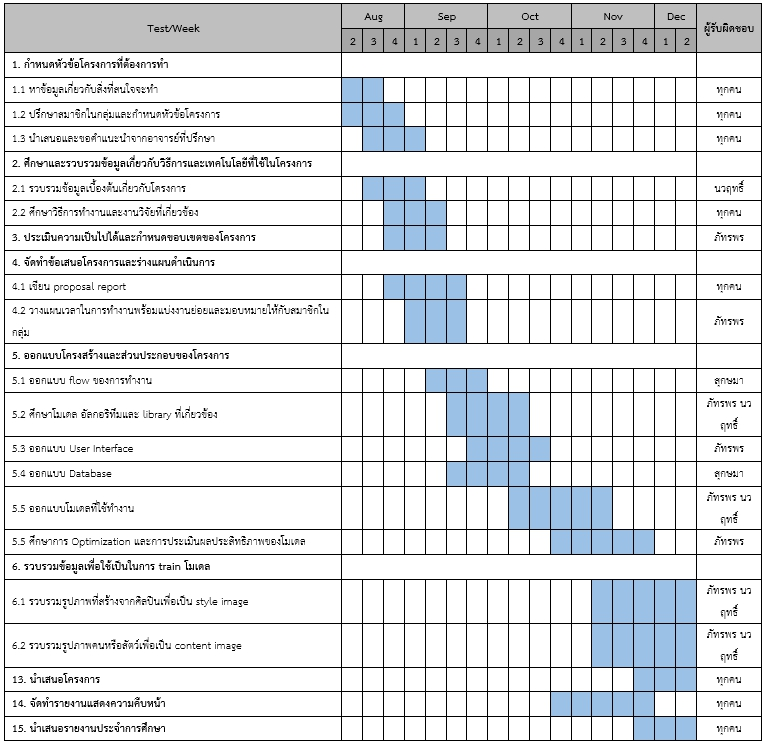
\includegraphics[width=15cm]{./image/plan_table1.jpg}
  \hfill
  \end{tabular}
\caption{ตารางแผนการทำงานภาคการศึกษาที่ 1\centering}
\label{tbl:plan1}
\end{table}

\newpage

\begin{table}[!h]
  \centering
  \begin{tabular}{c}
  \hfill
  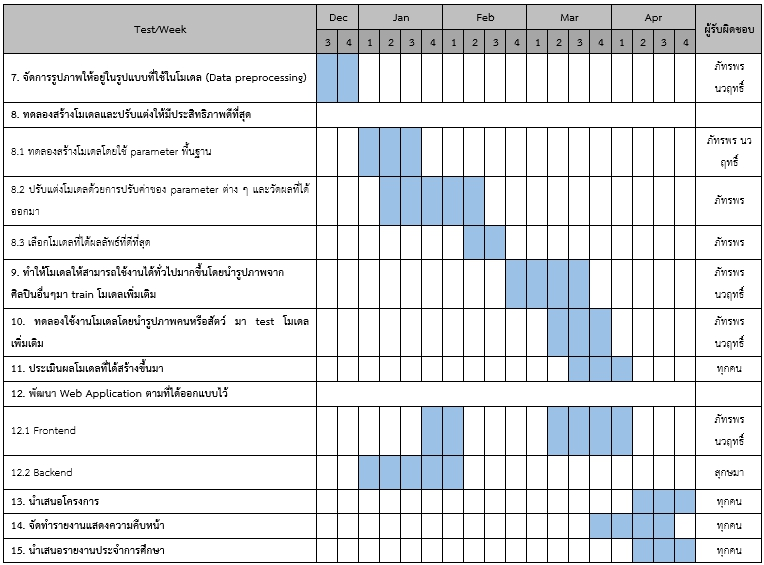
\includegraphics[width=15cm]{./image/plan_table2.jpg}
  \hfill
  \end{tabular}
\caption{ตารางแผนการทำงานภาคการศึกษาที่ 2\centering}
\label{tbl:plan2}
\end{table}


\section{ผลการดำเนินการ}
\subsection{ผลการดำเนินการในภาคการศึกษาที่1}
\begin{enumerate}
  \item ศึกษาและรวบรวมข้อมูลเกี่ยวกับวิธีการและเทคโนโลยีที่ใช้ในโครงการ
  \item ประเมินความเป็นไปได้และกำหนดขอบเขตของโครงการ
  \item จัดทำข้อเสนอโครงการและร่างแผนดำเนินการ
  \item ออกแบบโครงสร้างและส่วนประกอบของโครงการ
  \item รวบรวมข้อมูลเพื่อใช้เป็นในการ train โมเดล (style image และ content image)
  \item จัดการรูปภาพให้อยู่ในรูปแบบที่ใช้ในโมเดล (Data preprocessing)
  \item สร้างโมเดลโดยใช้ parameter พื้นฐาน
  \item จัดทำรายงานแสดงความคืบหน้า
\end{enumerate}

\newpage
\subsection{ผลการดำเนินการในภาคการศึกษาที่2}
\begin{enumerate}
  \item ทดลองสร้างโมเดลและปรับแต่งให้มีประสิทธิภาพดีที่สุด
  \item ทำโมเดลให้สามารถใช้งานได้ทั่วไปมากขึ้น
  \item ทดลองใช้งานโมเดล
  \item จัดทำ Web application ตามที่ออกแบบไว้
  \item นำเสนอโครงการ
  \item จัดทำรายงานแสดงความคืบหน้า
  \item นำเสนอรายงานประจำการศึกษา
\end{enumerate}


%%%%%%%%%%%%%%%%%%%%%%%%%%%%%%%%%%%%%%%%%%%%%%%%%%%%%%%%%%%%
%%%%%%%%%%%%%%  Literature Review %%%%%%%%%%%%%%%%%%%%%%%%%%
%%%%%%%%%%%%%%%%%%%%%%%%%%%%%%%%%%%%%%%%%%%%%%%%%%%%%%%%%%%%
\chapter{ทฤษฎีความรู้และงานที่เกี่ยวข้อง}
\section{บทนำ}
\par\setlength{\parindent}{5ex}ในบทนี้ อธิบายเกี่ยวกับแนวคิดที่นำมาประยุกต์ใช้ในโครงงาน อัลกอริทึมที่ใช้ในการทำโครงงานคือ VGGNet และมีการพัฒนาโดยใช้ภาษา python นอกจากนี้มีการทบทวนวรรณกรรม ที่จะกล่าวถึงโครงงานที่มีลักษณะเนื้อหาที่เกี่ยวข้องกับการทำโครงการนี้

\section{แนวความคิดทางทฤษฎี}
\subsection{Neural style transfer}
\par\setlength{\parindent}{5ex}Neural Style Transfer \cite{saha2018comprehensive} เป็นกระบวนการที่ใช้ CNNs ในการประมวลผลรูปภาพให้ได้รูปภาพที่เหมือนกับรูปภาพที่ใช้เป็น content image 
แต่มีรูปแบบหรือลักษณะที่ต่างกันไปตามรูปภาพที่ใช้เป็น style image ดังรูปที่~\ref{fig:modelcnn}


\begin{figure}[!h]
  \centering
  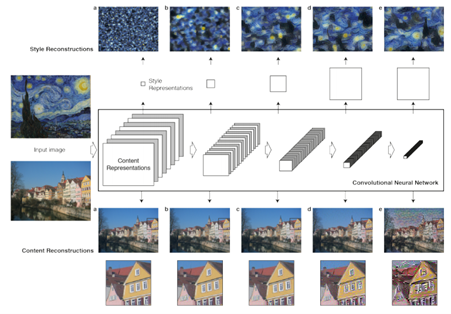
\includegraphics[width=10cm]{./image/unit1.png}
  \caption{แสดงหลักการทำงานของ Neural Style Transfer ที่ใช้ Convolutional Neural Network (CNN) \cite{gatys2015neural} }
  \label{fig:modelcnn}
\end{figure}

\par\setlength{\parindent}{5ex}
ดังรูปที่~\ref{fig:modelcnn} จะเห็นได้ว่า มีการป้อนข้อมูลเป็น content image และ style image 
จากนั้นจะการประมวลผลรูปที่ป้อนเข้ามา โดยจะมี filters ที่ reconstruct 
รูปภาพทั้ง content และ style โดยแสดงให้เห็นกระบวนการต่าง ๆ ใน CNN layer ต่าง ๆ 
ได้แก่ conv1\textunderscore1(a), conv2\textunderscore1(b), conv3\textunderscore1(c), conv4\textunderscore1(d) และ conv5\textunderscore1(e) 
ซึ่งจะเห็นว่า ใน layer หลัง ๆ รูปภาพที่ได้รูปภาพที่ได้มีการลดทอนของรูปภาพที่เป็น content 
และมีการเพิ่มส่วนของรูปภาพที่เป็น style เข้าด้วยกัน จนได้ได้รูปภาพที่เหมือนกับรูปภาพที่ใช้เป็น content image 
แต่มีรูปแบบหรือลักษณะที่ต่างกันไปตามรูปภาพที่ใช้เป็น style image

\subsection{Overview of machine learning}
\par\setlength{\parindent}{5ex}Machine learning (ML) เป็นการทำให้คอมพิวเตอร์สามารถเรียนรู้ได้ด้วยตนเอง โดยเริ่มต้นจะต้องสอนให้คอมพิวเตอร์เข้าใจก่อน โดยมีรูปแบบการเรียนรู้ 3 แบบ คือ  Supervised Learning เป็นการเรียนรู้ที่สอนให้คอมพิวเตอร์รู้จักทั้งข้อมูลที่เป็น input และ output ตัวอย่างเช่น การทำนายรูปภาพว่าเป็นหมาหรือแมว ซึ่งต้องสอนให้คอมพิวเตอร์รู้ว่ารูปภาพนี้เป็นหมาหรือแมวก่อนถึงจะเอาไปใช้ได้ เป็นต้น, Unsupervised Learning เป็นการเรียนรู้ที่สอนคอมพิวเตอร์เฉพาะข้อมูลที่เป็น input ไม่มี output ให้โดยจะให้คอมพิวเตอร์เรียนรู้ input ไปเรื่อย ๆ ตัวอย่างเช่น การจัดกลุ่มข้อมูล โดยจะป้อนเฉพาะข้อมูลเข้าไปแล้วคอมพิวเตอร์จะเรียนรู้เองว่า ข้อมูลแบบนี้ควรอยู่กับข้อมูลแบบไหน เป็นต้นและ Reinforcement learning ที่เป็นการเรียนรู้โดยการปฏิสัมพันธ์กับสิ่งแวดล้อมรอบ ๆ โดยถ้าทำถูกต้องจะได้คะแนนเพิ่ม ถ้าทำผิดคะแนนจะลดลง ตัวอย่างเช่น การเดินไปข้างหน้าของหุ่นยนต์ที่จะต้องรู้ก่อนว่า อยู่ตำแหน่งไหน แล้วในตำแหน่งควรเดินไปตำแหน่งไหนต่อไปถึงจะดี เป็นต้น
\par\setlength{\parindent}{5ex}ในขั้นตอนการสร้างโมเดล machine learning จะมีข้อมูล input ที่เกี่ยวข้อง 2 ส่วนคือ training set เป็นชุดข้อมูลที่ใช้สำหรับการสอนโมเดลโดยจะฝึกฝนโมเดลให้ได้ผลลัพธ์ตามชุดข้อมูลที่ป้อนเข้ามา อีกส่วนคือ testing set เป็นชุดข้อมูลที่ใช้ทดสอบการทำงานของโมเดล โดยโมเดลที่ดีจะต้องไม่ทำให้เกิดการ overfitting หรือสามารถทำนายผลลัพธ์ใน training set ได้แม่นยำ แต่ทำนายผลลัพธ์ใน testing set ได้แย่ 
\par\setlength{\parindent}{5ex}เมื่อสอนคอมพิวเตอร์เรียบร้อยแล้ว เมื่อมีข้อมูลใหม่ ๆ เข้า คอมพิวเตอร์ก็สามารถจัดการหรือทำนายข้อมูลนั้นได้เลย ไม่จำเป็นต้องเขียนโปรแกรมใหม่ทุกครั้งที่มีข้อมูลเข้ามา

\subsection{Classical artificial neural networks}
\par\setlength{\parindent}{5ex}
Artificial neural networks(ANN) คือโมเดลทางคณิตศาสตร์หรือโมเดลทางคอมพิวเตอร์ที่จำลองการทำงานของเซลล์ประสาทในสมองมนุษย์ที่มีเซลล์ประสาท(neurons) และจุดประสาทประสาท  ดึงเกิดเป็น ANN ซึ่งมีส่นประกอบในการทำงาน 3 ส่วนหลัก ๆ ดังรูปที่~\ref{fig:cnn} คือ input layer, hidden layer และ output layer ซึ่งการทำงานของ artificial neural networks จะมี 2 ส่วนคือ กระบวนการทำงานไปข้างหน้าหรือ feed forward คือป้อน input เข้าไป แล้วเข้า hidden layer ทำการประมวลผลแล้วได้ค่าออกมาส่งไปที่ output layer และ back propagation หรือกระบวนการทำย้อนกลับโดยจะเป็นการทำย้อนกลับจาก output layer ไป input layer

%%%%%%%no ref
\begin{figure}[!h]
  \centering
  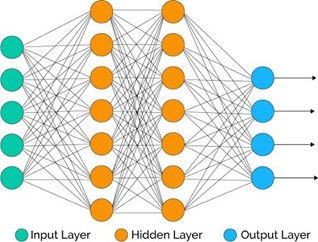
\includegraphics[width=8cm]{./image/unit2.jpg}
  \caption{แสดงส่วนประกอบหลักของ Artificial neural networks}
  \label{fig:modelann}
\end{figure}

\par\setlength{\parindent}{5ex}
ในแต่ละ layer จะมีก้อนกลม ๆ อยู่หรือก็คือ neuron unit อยู่ดังรูปที่~\ref{fig:modelann} ถ้าใน input layer ภายในจะเก็บข้อมูลที่รับเข้ามา แต่ถ้าเป็น hidden layer ภายในจะมีการคำนวณเกิดขึ้นโดยสามารถเพิ่ม hidden layer ได้หลาย layer ตามที่ผู้พัฒนาต้องการได้ ส่วนใน output layer จะมีการทำนายผลออกมาว่า ผลที่ได้เป็นคลาสอะไร


\subsubsection{Neuron unit ใน hidden layer}
\par\setlength{\parindent}{5ex}
ภายใน neuron unit แต่ละตัวใน hidden layer จะมีการคำนวณโดยหลังจากผ่าน input layer เข้ามาจะมีการเพิ่ม weight ให้กับ input neuron unit แต่ละตัว จากนั้นเมื่อเข้า hidden layer ภายในจะรวมผลคูณระหว่าง weight กับ input neuron unit แต่ละตัวเข้าด้วยกันแล้วเข้า step function หรือส่วนใหญ่เรียกว่า activation function 
จากนั้นจะได้ output ออกมา ดังรูปที่~\ref{fig:modelNU}

%%%%%%%no ref
\begin{figure}[!h]
  \centering
  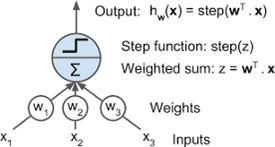
\includegraphics[width=8cm]{./image/neuron_unit.png}
  \caption{แสดงการทำงานภายใน neuron unit \cite{DeepLear55:online}}
  \label{fig:modelNU}
\end{figure}

\subsubsection{Backward propagation}
\par\setlength{\parindent}{5ex}
Backward propagation เป็นกระบวนการทำงานย้อนกลับจาก output layer มา input layer เพื่อปรับค่า weight แต่ละตัวให้ดีขึ้น โดยจะทำไปเรื่อง ๆ จนกว่าจะได้ cost function หรือ error ที่น้อยตามที่ต้องการ 
โดยลักษณะการทำงานของ feed forward กับ back propagation มีลักษณะต่างกันดังรูปที่~\ref{fig:feed-back}

\begin{figure}[!h]
  \centering
  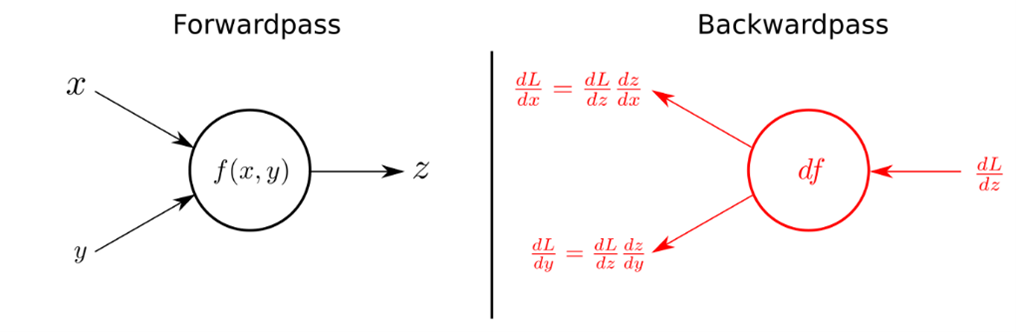
\includegraphics[width=8cm]{./image/feed_back.png}
  \caption{แสดงการทำงานของ feed forward (forwardpass) กับ back propagation (backwardpass)}
  \label{fig:feed-back}
\end{figure}

\par\setlength{\parindent}{5ex}
ในการทำ back propagation จะใช้อัลกอริทึม optimization เพื่อเพิ่มประสิทธิภาพตัวนึงที่ชื่อว่า Gradient descent algorithm \cite{Gradient17:online} ที่จะทำการหา weight ที่ต่ำที่สุดที่จะทำให้โมเดลสามารถทำนายผลได้ดีที่สุด เกิด error น้อย

\subsubsection{Cost function}
\par\setlength{\parindent}{5ex}
Cost function หรือ loss function หรือค่า error ที่เกิดขึ้น ซึ่งจุดมุ่งหมายของโมเดลต่าง ๆ จะเหมือนกันคือ ต้องการให้เกิดค่า error ที่น้อยที่สุดที่เป็นไปได้ ซึ่งการคำนวณค่า error ที่เกิดขึ้นจะใช้การเปรียบเทียบระหว่างผลลัพธ์จริง ๆ ที่ได้มาจากข้อมูลจริงกับผลลัพธ์ที่เกิดจากการทำนายโดยโมเดลมาเทียบกันโดยใช้วิธีต่าง ๆ ตัวอย่างเช่น การคำนวณค่า Mean Squared Error Loss, Mean Absolute Error Loss, Binary Crossentropy Loss, Categorical Crossentropy Loss, Sparse Categorical Crossentropy Loss เป็นต้น ซึ่งการคำนวณแบบต่าง ๆ ก็เหมาะกับปัญหาคนละแบบ ตัวอย่างเช่น Binary Crossentropy Loss ที่เหมาะกับข้อมูลที่มีเพียง 2 คลาส เป็นต้น

\subsection{Convolutional Neural Network (CNN)}
\par\setlength{\parindent}{5ex}
Convolutional Neural Network (CNN) หรือ ConvNet  \cite{WhatisWe89:online,NeuralTr45:online} เป็นอัลกอริทึม Deep Learning 
ชนิดหนึ่งที่ใช้ประมวลผลรูปภาพ โดยเรียนรู้คุณลักษณะต่าง ๆ ของรูปภาพที่ป้อนเข้าผ่านการใช้ filters 
ซึ่งเป็นการเรียนรู้ลักษณะของรูปภาพ เพื่อแยกแยะว่า รูปภาพที่ป้อนเข้ามาเป็นรูปอะไรดังรูปที่~\ref{fig:pic-cnn}

\begin{figure}[!h]
  \centering
  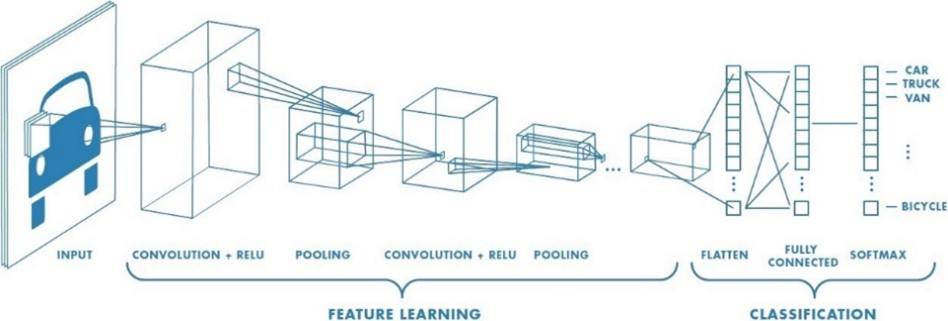
\includegraphics[width=12cm]{./image/cnn.jpg}
  \caption{แสดงให้เห็นถึงกระบวนการทำงานของ CNN ที่มีการเรียนรู้ 2 ส่วนคือ feature learning ซึ่งมี convolution layer และ pooling layer ประกอบกัน และ classification ซึ่งมี fully connected layer มาเกี่ยวข้อง}
  \label{fig:pic-cnn}
\end{figure}


\subsubsection{Input data}
\par\setlength{\parindent}{5ex}
ข้อมูลที่เข้ามาประมวลใน CNN เป็นรูปภาพซึ่งมีหลากหลายรูปแบบที่เป็นขาวดำหรือ Grayscale, รูปภาพสีแบบ RGB, HSV หรือ CMYK เป็นต้น ซึ่งโดยส่วนใหญ่เป็นรูปภาพสีแบบ RGB ซึ่งเมื่อรับ input เข้ามาจะถูกแบ่งสีออกเป็น channels คือ Red(R) , Green(G) และ Blue(B) และแปลงขนาดความกว้างและความยาวของรูปภาพให้เป็น pixels 
ทำให้อยู่ในรูป heights*weights*จำนวนของ channels ดังรูปที่~\ref{fig:rgb-layer}

\begin{figure}[!h]
  \centering
  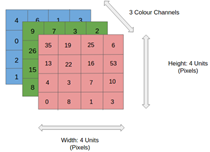
\includegraphics[width=8cm]{./image/unit3.png}
  \caption{แสดงให้เห็นถึงลักษณะของ input data ที่มีการแบ่งชั้นสีเป็น 3 channels ซึ่งจากรูปนี้จะมีขนาดของรูปเป็น 4*4*3 RGB Image}
  \label{fig:rgb-layer}
\end{figure}

\subsubsection{Convolution layer}
\par\setlength{\parindent}{5ex}
ในส่วนของ convolutional layer จะมี filter หรือ Kernel (K) ซึ่งเป็น matrix ขนาดต่าง ๆ ใช้สำหรับ map กับข้อมูลที่เข้ามา และมี stride ที่ใช้สำหรับบอกว่าต้องขยับ filter ไปกี่ pixels โดย filters จะเคลื่อนที่ไปเรื่อย ๆ จนผ่านครบทุก pixels ในข้อมูลที่เข้ามา และนอกจากนี้จะมีการใช้ non-linear functions เพื่อ scale ข้อมูลที่เข้ามาไม่ให้ติดลบซึ่งเหมาะกับการเรียนรู้ใน CNNs โดยตัวที่นิยมใช้คือ Rectified Linear Unit (ReLU) ที่มีฟังก์ชันคือ ƒ(x) = max(0,x) 

\subsubsection{Pooling layer}
\par\setlength{\parindent}{5ex}
ในส่วนของ pooling layer จะทำงานต่อจาก convolution layer โดยจะทำการดึงข้อมูลออกมาหลังจากที่มีการทำ filter แต่ละครั้ง ออกมาเป็นข้อมูลที่ออกมา ณ ตำแหน่งนั้น ๆ ที่มีการทำ filter ทำให้สามารถดึงลักษณะสำคัญของข้อมูลที่เข้ามาได้ ตัวอย่างเช่น ขอบ สี รูปทรง เป็นต้น และยังทำให้ขนาดข้อมูลที่ได้ออกมามีขนาดเล็กลงเมื่อเทียบกับข้อมูลที่เข้ามา โดย pooling มี 3 แบบ คือ min pooling, max pooling และ average pooling ซึ่ง convolution layer กับ pooling layer จะทำงานคู่กัน ซึ่งใน CNN จะมีกี่ layer นั้นขึ้นอยู่กับความซับซ้อนของรูปภาพ

\subsubsection{Fully connected layer}
\par\setlength{\parindent}{5ex}
เมื่อทำ feature learning โดยใช้ convolution layer กับ pooling layer แล้ว output ที่ได้จะอยู่ในรูปแบบที่เป็น 3 ชั้นหรือมี 3 มิติอยู่ จะมีการทำ flatten ก่อนเพื่อให้อยู่ในรูปแบบที่เป็น 1 มิติ เพื่อที่จะได้สามารถเข้าไปใน fully connected layer ได้ โดยใน fully connected layer มีการใช้ softmax classification ที่ใช้แยกว่าข้อมูล input ที่เข้ามาเป็นรูปอะไรโดยแสดงผลเป็นความเป็นไปได้ที่เป็นรูปต่าง ๆ 

\subsection{Transfer Learning}
\par\setlength{\parindent}{5ex}
Transfer Learning เป็นการเรียนรู้ที่เป็นที่นิยมในการทำ machine learning(ML) โดยเป็นการนำโมเดลที่มีคนสร้างมาก่อนที่เหมาะกับงานหนึ่ง ๆ มาประยุกต์ใช้กับงานอื่นโดยไม่จำเป็นต้องสอนโมเดลใหม่ทั้งหมด 
ทำให้สามารถลดเวลาประมวลผลและเวลาในการสอนโมเดลได้ ดังรูปที่~\ref{fig:ml-tl}

\newpage

\begin{figure}[!h]
  \centering
  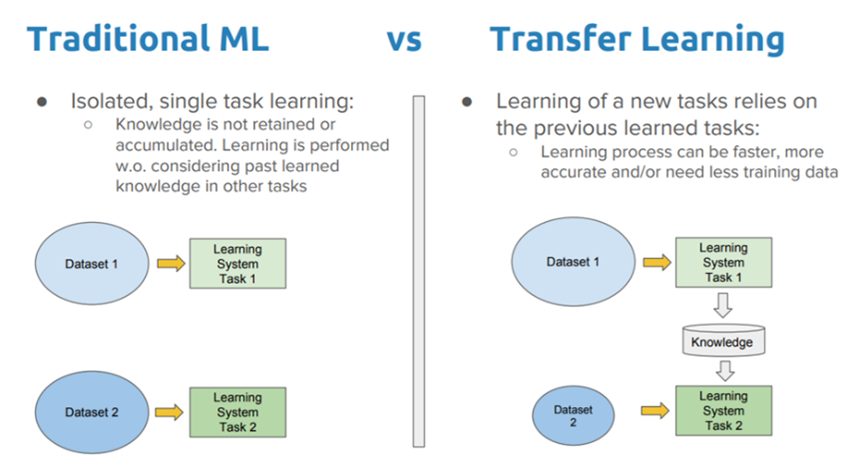
\includegraphics[width=12cm]{./image/unit4.png}
  \caption{แสดงให้เห็นถึงการเปรียบเทียบการทำงานระหว่าง traditional ML กับ transfer learning ที่มีรูปแบบการทำงานที่ต่างกัน \cite{brownlee2017gentle}}
  \label{fig:ml-tl}
\end{figure}

\par\setlength{\parindent}{5ex}
โดยในการทำ transfer learning มีอยู่ 2 รูปแบบ คือ develop model ซึ่งเป็นการนำโมเดลนั้นมาแก้ไขและพัฒนาให้ดีกว่าเดิมให้เหมาะกับงานที่โมเดลนั้นสร้างมาใช้และจึงนำไปใช้กับงานอื่น ๆ ส่วนอีกรูปแบบคือ pre-trained model ซึ่งเป็นการนำโมเดลไปใช้กับงานอื่นเลย โดยส่นใหญ่จะใช้ pre-trained model เป็นหลัก 
\par\setlength{\parindent}{5ex}
สำหรับการทำ transfer learning ที่เกี่ยวกับรูปภาพ\cite{8636278}\cite{sarkar2018comprehensive}มีการสร้างโมเดลสำหรับ ImageNet ที่มีรูปภาพกว่า 1.4 ล้านรูปและมากกว่า 1,000 คลาสที่เป็นความท้าทายสำหรับการทำ image classification ทำให้มีองค์การวิจัยต่าง ๆ มีการพัฒนาโมเดลขึ้นมาสำหรับแก้ปัญหานี้ และได้เปิดให้คนทั่วไปสามารถเอาไปใช้ได้ ตัวอย่างเช่น โมเดล VGG ของ Oxford, โมเดล Inception ของ Google และโมเดล ResNet ของ Microsoft เป็นต้น

\subsubsection{VGGNet}
\par\setlength{\parindent}{5ex}
Visual Geometry Group (VGG) เป็น CNN สำหรับจดจำรูปภาพ ซึ่งสถาปัตยกรรมของ VGG จะประกอบไปด้วยบล็อค 
แต่ละบล็อกจะเป็น 2 มิติ คือ Convolution layer และ Pooling layer แนวความคิดนี้ถูกพัฒนาโดย 
Simonyan \& Zisserman จาก Oxford Robotics Institute ซึ่ง VGG นั้นมีโมเดล 2 ตัวคือ VGG16 และ VGG19 
ซึ่งเลข 16 และ เลข 19 นั้นมาจากคือจำนวนของ hidden layer สำหรับ VGG16 จะประกอบไปด้วยบล็อคของ 
convolutional layer และ Pooling ทั้งหมด 13 layers และ Fully connected layer 3 layers ส่วน VGG 19 
นั้นคือ VGG16 ที่มีบล็อคของ convolutional layer เพิ่มมาอีก 3 layers  ดังรูปที่ ~\ref{fig:vgg16-19} 

\begin{figure}[!h]
  \centering
  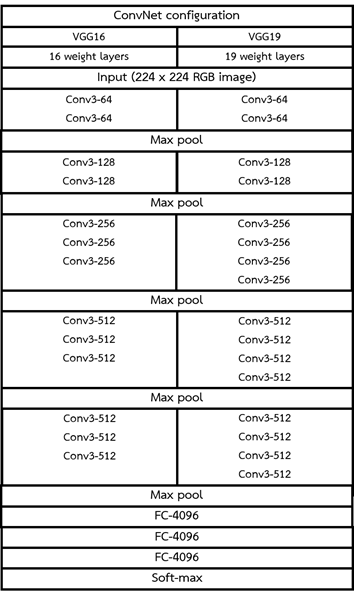
\includegraphics[width=8cm]{./image/vgg16-19.png}
  \caption{แสดงสถาปัตยกรรมของ VGG16 และ VGG19}
  \label{fig:vgg16-19}
\end{figure}

\newpage

\subsection{Web Application}
\par\setlength{\parindent}{5ex}
Web Application เป็นซอฟต์แวร์นึงที่สามารถเข้าถึงผ่าน browser ใดก็ได้ โดยที่ผู้ใช้ไม่ต้องดาวน์โหลดก่อนใช้งานเพราะสามารถเข้าถึงได้ผ่าน network ซึ่ง Web Application นั้นออกแบบมาให้สามารถมีปฏิสัมพันธ์กับผู้ใช้ได้ ไม่ใช่แค่การดูข้อมูลต่าง ๆ แต่สามารถจัดการหรือใช้งานได้ ซึ่งผู้ใช้หลายคนสามารถเข้าถึงพร้อมกัน
\par\setlength{\parindent}{5ex}
หลักการทำงานของ web Application คือ ผู้ใช้งานติดต่อสื่อสารกับ web application ผ่าน frontend หรือ client-side ซึ่ง frontend จะมีการเรียกใช้หรือดึงข้อมูลออกมาจาก backend หรือ server-side ผ่าน http request ที่ถูกเรียกใช้โดยผู้ใช้งาน ภายใน backend จะมี web server, database 
และไฟล์อื่น ๆ เก็บไว้ ดังรูปที่~\ref{fig:webapp} 

%%%%no ref
\newpage
\begin{figure}[!h]
  \centering
  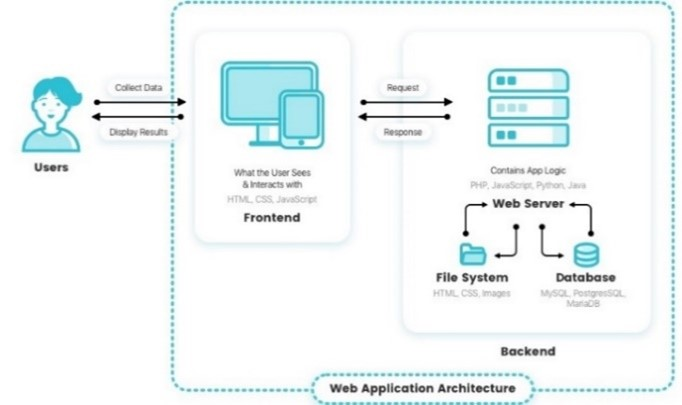
\includegraphics[width=8cm]{./image/webapp.jpg}
  \caption{แสดงหลักการทำงานของ web application}
  \label{fig:webapp}
\end{figure}

\subsection{Development Tools}
\subsubsection{Python}
\par\setlength{\parindent}{5ex}
Python เป็นภาษาที่ใช้ในการเขียนโปรแกรม ซึ่งได้รับความนิยมเป็นอย่างมาก เนื่องจากเป็นภาษาที่เรียนรู้ง่าย ใช้งานง่ายและมีประสิทธิภาพสูง ถูกพัฒนาขึ้นโดย Guido van Rossum ในปี ค.ศ. 1991 ซึ่งสามารถทำงานบนแพลตฟอร์ต่าง ๆ ได้หลากหลาย มีไวยากรณ์ที่เข้าใจง่ายสามารถเขียนได้ทั้งแบบเชิงวัตถุ object-oriented หรือแบบฟังก์ชัน functional และรันบน interpreter system ซึ่งประมวลผลได้อย่างรวดเร็วและมี library หลากหลายให้ใช้งาน

\subsubsection{Hypertext Markup Language (HTML)}
\par\setlength{\parindent}{5ex}
Hypertext Markup Language (HTML) เป็นภาษาคอมพิวเตอร์ที่ใช้ในการแสดงผลของข้อความ รูปภาพหรือวัตถุอื่น ๆ บนหน้าเว็บไซต์ โดยมีโครงสร้างการเขียนที่อาศัย tag ควบคุมซึ่งถูกพัฒนาโดย World Wide Web Consortium (W3C) โดยออกแบบมาให้สามารถทำความเข้าใจและเรียนรู้ง่าย โดยใน tag ต่าง ๆ จะแตกต่างกันไปแต่มีส่วนประกอบหลักที่เหมือนกันคือ เครื่องหมาย “<>” และมีชื่ออยู่ตรงกลางเครื่องหมายนั้น ตัวอย่างเช่น <head> </head> เป็นต้น

\subsubsection{Cascading Style Sheets (CSS)}
\par\setlength{\parindent}{5ex}
Cascading Style Sheets (CSS) หรือ Style Sheets เป็นภาษาคอมพิวเตอร์ตัวนึง ที่ใช้สำหรับกำหนดรูปแบบการแสดงผลของเอกสาร html อันได้แก่ สีข้อความ ขนาดข้อความ ประเภทตัวอักษร ขนาดรูปภาพ การจัดวางข้อความ สีพื้นหลัง เป็นต้น

\subsubsection{JavaScript}
\par\setlength{\parindent}{5ex}
JavaScript เป็นภาษาคอมพิวเตอร์ชนิดหนึ่งที่ใช้ร่วมกับเอกสาร html เพื่อให้เว็บไซต์มีการเคลื่อนไหวเพื่อตอบสนองต่อการใช้งานของผู้ใช้มากขึ้น โดยมีลักษณะการทำงานคือ แปลความและดำเนินงานไปทีละคำสั่ง หรือ object-oriented programming ซึ่งดำเนินการโดย browser เป็น client-side script ทำให้สามารถใช้งานกับ server ใดก็ได้ โดย javaScript นี้สามารถเขียนเพื่อเปลี่ยนแปลง html element ได้ สามารถตอบสนองกับผู้ใช้และตรวจสอบข้อมูล รวมไปถึงสร้าง cookies ที่ใช้เก็บข้อมูลในคอมพิวเตอร์ของผู้ใช้ได้

\subsubsection{Pytorch}
\par\setlength{\parindent}{5ex}
Pytorch เป็น Deep learning library ที่ Facebook เป็นคนพัฒนาขึ้นด้วยภาษา python โดยดัดแปลงมาจาก library torch ที่ถูกใช้ในภาษา Lua มาก่อน โดยจะมองข้อมูลให้อยู่ในรูปของ tensor ซึ่งเป็นการเก็บข้อมูลหลายมิติแบบ arrays ทำให้สามารถใช้ numpy ในการคำนวณได้เลย และมีการเตรียม neural network แบบต่าง ๆ ไว้ให้ผู้พัฒนาสามารถนำไปพัฒนาต่อได้อย่างรวดเร็ว และยังสามารถใช้ GPU เข้ามาช่วยในการคำนวณได้ ทำให้สามารถประมวลผลได้เร็วขึ้น

\subsubsection{Django}
\par\setlength{\parindent}{5ex}
Django เป็น high-level python web framework ที่ช่วยให้ผู้พัฒนาสามารถสร้าง web application ได้อย่างรวดเร็ว ซึ่งจุดเด่นของ Django คือ มีระบบ admin มาให้ทำให้ผู้พัฒนาไม่จำเป็นสร้างใหม่เอง สามารถใช้งานกับโปรแกรม editor ได้หลากหลายตามที่ผู้พัฒนาถนัด มีเครื่องมือที่ช่วยให้ผู้พัฒนาสามารถขึ้นโครงโปรแกรมได้อย่างรวดเร็ว ตัวอย่างเช่น ระบบการจัดการข้อมูล(models), ระบบแสดงผล(views), ระบบการเข้าใช้งานของผู้ใช้, ระบบการจัดการผู้ใช้งาน เป็นต้น รวมทั้งมี Django REST Framework ที่ช่วยให้ผู้พัฒนาสามารถสร้าง API เพื่อให้ในส่วน frontend สามารถติดต่อกับส่วน backend ได้อย่างสะดวก รวดเร็ว

\par\setlength{\parindent}{5ex}
หลักการของ Django คือ 1 Project มี 1 app โดย 1 app คือ 1 module ในเว็บไซต์ ในการสร้าง Django Project \cite{ปูพื้นฐา98:online} ผู้ใช้จะได้ไฟล์หลายไฟล์ดังรูปที่ 2.10 ซึ่งไฟล์หลัก ๆ ประกอบไปด้วย
\begin{enumerate}
  \item manage.py ที่เป็นไฟล์ script สำหรับรันคำสั่งต่าง ๆ ที่เกี่ยวข้องกับ Django
  \item \textunderscore init\textunderscore.py เป็นไฟล์ initial หรือไฟล์เปล่าที่มีไว้สำหรับเก็บ package ของ python
  \item setting.py เป็นไฟล์ที่ใช้ตั้งค่า project ตัวอย่างเช่น การตั้งค่า app, การตั้งเวลา, การตั้งค่า path เป็นต้น
  \item urls.py เป็นไฟล์ที่มีไว้สำหรับเก็บ HTTP Request หรือ url pattern ที่เป็นการ routing ภายใน Django project
  \item wsgi.py เป็นไฟล์ที่เก็บข้อมูลสำหรับการ deployment หรือการ production ให้ผู้ใช้ใช้งาน
\end{enumerate}



\begin{figure}[!h]
  \centering
  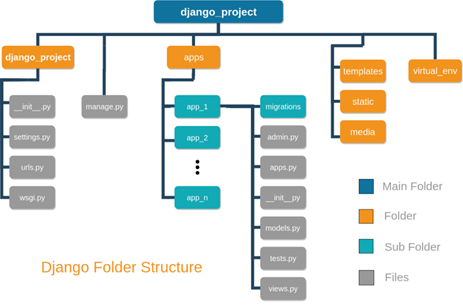
\includegraphics[width=8cm]{./image/django.png}
  \caption{แสดงโครงสร้างโฟลเดอร์ของ Django project}
  \label{fig:django}
\end{figure}

\par\setlength{\parindent}{5ex}
และ Django เป็น model-view-template (MVT) ซึ่งมีกระบวนการทำงานหลัก ๆ 3 ส่วน ดังรูปที่~\ref{fig:django2} คือ Model ที่เก็บข้อมูลของ application, View สำหรับประมวลผลคำสั่งหรือข้อมูลต่าง ๆ แล้วส่งไปที่ Template, Template คือหน้า application ที่ใช้แสดงผลข้อมูลที่ผ่านการประมวลผลจาก view ร่วกับ html โดยมีการใช้ http request และ http response ในการติดต่อกับส่วนต่าง ๆ 

%%%%%no ref
\begin{figure}[!h]
  \centering
  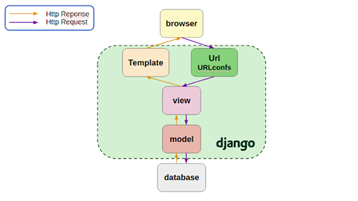
\includegraphics[width=8cm]{./image/django2.png}
  \caption{แสดงกระบวนการทำงานของ Django}
  \label{fig:django2}
\end{figure}


\subsubsection{MongoDB}
\par\setlength{\parindent}{5ex}
MongoDB เป็นฐานข้อมูลแบบ NoSQL ที่เป็น open source ชนิดหนึ่ง ซึ่งเก็บข้อมูลแบบไม่มีความสัมพันธ์กันซึ่งต่างจากการเก็บข้อมูลแบบ SQL ทั่วไปทำให้ไม่จำเป็นต้องกำหนดโครงสร้างใด ๆ โดยจะมีโครงสร้างแบบ document database ที่เก็บข้อมูลในรูปแบบ JSON (JavaScript Object Notation) ซึ่งมี key และ value โดยจะเก็บข้อมูลใน collection ต่าง ๆ และเรียกแถวเป็น document และคอลัมภ์เป็น field เนื่องจากไม่มีโครงสร้างใด ๆ ทำให้สามารถอ่านและเขียนได้อย่างรวดเร็ว

\section{การทบทวนวรรณกรรม}
\par\setlength{\parindent}{5ex}
งานวิจัยเรื่อง A Neural Algorithm of Artistic Style ของ Gatys  et al.\cite{gatys2015neural} ซึ่งทำการศึกษาการเอารูปภาพ (Content Image) ไปรวมกับรูปแบบ Artwork (Style Image) ของอีกภาพหนึ่ง โดยใช้ภาพ content Style จาก Neckarfront ในเมือง Tubingen ประเทศเยอรมัน และ style image จาก 5 ภาพของศิลปิน ดังนี้ ภาพ the shipwreck of the minotaur ของ J.M.W. Turner ภาพ The starry night ของ Vincent van Gogh ภาพ Der Schrei ของ Edvard Munch ภาพ Femme nue assise ของ Pablo Picasso และ ภาพ Composition ของ Wassily Kandinsky  และใช้  VGG-network  ที่มี 16 convolutional layers และ 5 pooling layers ของ VGG19 ในงานวิจัยนี้ไม่ได้ใช้ full connected layer และเลือกใช้ average pooling แทนที่ max-pooling 
\par\setlength{\parindent}{5ex}
งานวิจัยเรื่อง Stable and controllable neural texture synthesis and style transfer using histogram loss ของ Risser et al. ได้เห็นปัญหาจากวิธีของ Gatys et al. ที่มีข้อจำกัดในเรื่อง texture quality, stability, requisite parameter tunning และ lack of user control จึงเสนอให้ใช้ histogram loss แทนที่ gram loss ซึ่งพบว่าเมื่อใช้ histogram loss จะใช้ ประมาณ 700 iteration ในการประมวลผลแต่ละภาพ  (งานของ Gatys et al. ใช้ประมาณ 1000 iteration) แต่ภาพที่ได้จากงานวิจัยนี้มีความ stable กว่า 
\par\setlength{\parindent}{5ex}
งานวิจัยเรื่อง Two-stage color ink painting style transfer via convolution neural network ของ Zheng et al.\cite{8636278} งานวิจัยนี้ศึกษาวิธีการประมวลผลภาพวาดดอกไม้เป็นภาพวาดหมึกสี (color ink painting) ซึ่งเป็นภาพแบบดั้งเดิมของจีน (Traditional Chinese Painting) ซึ่งมีลักษณะการวาดที่แตกต่างกับภาพวาดทางตะวันตก งานวิจัยแบ่งวิธีการประมวลผลออกเป็น 2 งานย่อย คือ line drawing extraction และ image colorization โดยในส่วน line drawing extraction จะประมวลผลโดยใช้ CNN-based neural style transfer และในส่วนของ image colorization จะประมวลผลโดยใช้ GAN-based neural style transfer


\newpage





%%%%%%%%%%%%%%%%%%%%%%%%%%%%%%%%%%%%%%%%%%%%%%%%%%%%%
%%%%%%%%%%%%%%%%%%%%%%%%%%%%%%%%%%%%%%%%%%%%%%%%%%%%%
%%%%%%%%%%%%%%%%%%%%%%%%%%%%%%%%%%%%%%%%%%%%%%%%%%%%%
\chapter{วิธีการดำเนินงาน}
\section{บทนำ}
\par\setlength{\parindent}{5ex}
ในบทนี้ อธิบายเกี่ยวกับรายละเอียดของโครงงาน สถาปัตยกรรมที่เกี่ยวข้อง วิธีการจัดการข้อมูลว่า ข้อมูลที่นำมาใช้ในการทำโครงงานนี้มีลักษณะอย่างไร มีการใช้อัลกอริทึมใดในการประมวลผลและแนวทางการประเมินผลการทำงาน

\section{รายละเอียดของโครงงาน}

\subsection{การทบทวนวรรณกรรม}
\par\setlength{\parindent}{5ex} 
หลังจากการศึกษาจากงานวิจัย คณะผู้จัดทำได้ลอง download code ที่ implement จากมางานวิจัยของ Gatys et al. \cite{NeuralTr45:online} มาศึกษาขั้นตอนวิธีการทำ neural style transfer และได้ทดลองนำภาพจากศิลปินไทย 2 ท่าน ท่านละ 1 style พบปัญหาจากวิธีการทำ neural style transfer แบบนี้คือ ขนาดของ style image และ content image ต้องมีขนาดที่เป็นความกว้างและความยาวเท่ากัน ระยะเวลาในการรันค่อยข้างนาน ใช้เวลา 45 นาที สำหรับ 5000 iteration บนคอมพิวเตอร์ intel(R) Core(TM) i5-8300H CPU @2.30GHz RAM 8 GB และ nvidia geforce gtx 1060 GPU 6 GB ผลลัพท์ในการประมวลแสดงดังภาพต่อไปนี้

\begin{figure}[!h]
  \centering
  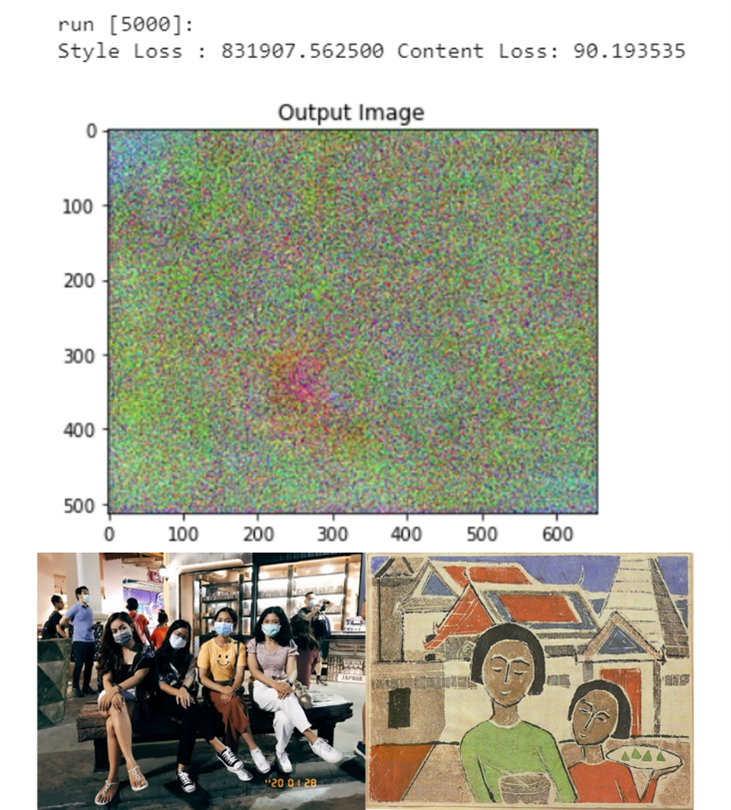
\includegraphics[width=10cm]{./image/result1.png}
  \caption{(บน) แสดงผลการประมวลผล (ล่างซ้าย) content image (ล่างขวา) style image: ชื่อภาพ ไปวัด ของชลูด นิ่มเสมอ}
  \label{fig:result1}
\end{figure}

\newpage
\begin{figure}[!h]
  \centering
  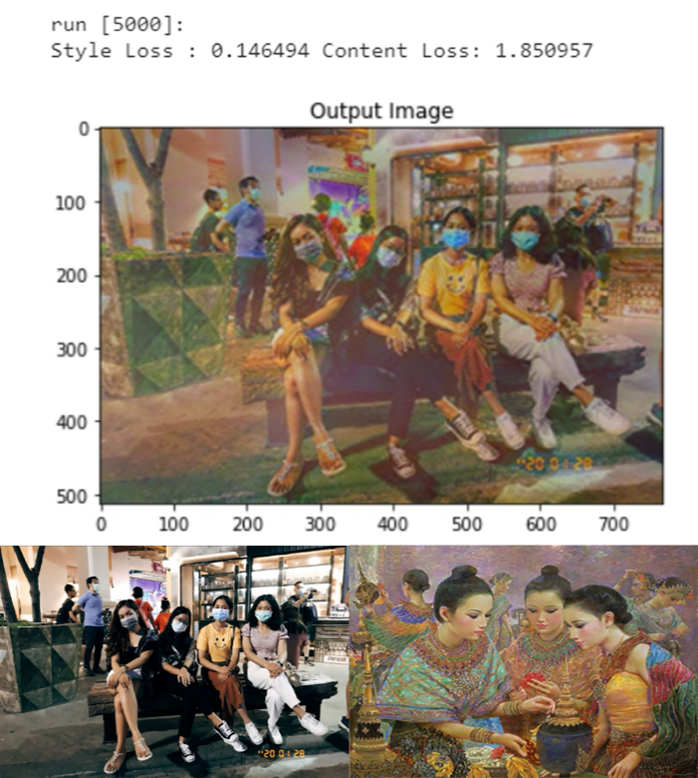
\includegraphics[width=10cm]{./image/result2.png}
  \caption{(บน) แสดงผลการประมวลผล (ล่างซ้าย) content image (ล่างขวา) style image: ชื่อภาพ ผูกอุบะของจักรพันธุ์ โปษยกฤต}
  \label{fig:result2}
\end{figure}

\subsection{Modeling}
\par\setlength{\parindent}{5ex}
สร้างโมเดลที่ใช้ input 2 ตัวคือ content image และ style image แล้วได้ output เป็นรูปภาพใหม่ที่รวมรูปแบบการวาดแบบ style image และมีเนื่อหาแบบ content image โดยได้พัฒนาโมเดลขึ้นมา ดังนี้

\begin{enumerate}
  \item ใช้โมเดล CNNs ในการแยกส่วนประกอบของรูปภาพ โดยทำ Transfer learning ด้วยการใช้ pre-trained โมเดล VGG19 
  \item ปรับเปลี่ยนโมเดล VGG19 ที่เดิมใช้ pooling layer จาก max pooling เป็น average pooling เนื่องจากถ้าใช้ max pooling ผลลัพธ์ที่ออกมาอาจทำให้บางจุดในรูปภาพมีสีที่โดดเด่นเกินไปจึงใช้  average pooling แทน
  \item มีการตัด layer สุดท้ายที่ใช้ในการแบ่งคลาสของ VGG19 ออกเนื่องจากไม่ได้ใช้และเพิ่ม layer ที่เป็น Upsampling layer และ convolutional layer เพื่อทำให้รูปภาพผลลัพธ์ที่ได้ออกมามีขนาดใหญ่ขึ้น จากเดิมที่ได้ขนาด 24*24*3 เป็น 224*224*3 เหมือนขนาดรูปที่เป็น input
  \item มีการปรับ weight layer ที่ใช้ โดยเมื่อเทียบกับโมเดลของ Gatys  et al. \cite{gatys2015neural} ที่ให้ weight ของ content layer ที่ layer เดียว (conv 4\textunderscore2) และให้ weight ของ style layer 5 layers (conv 1\textunderscore1, conv 2\textunderscore1, conv 3\textunderscore1, conv 4\textunderscore1, conv 5\textunderscore1) จะทำการปรับเป็นให้ weight ของ content layer 2 layers (conv 2\textunderscore2, conv 4\textunderscore2) และให้ weight ของ style layer 5 layers เหมือนเดิม 
  \item มีการปรับเปลี่ยนการใช้ gram matrics จากเดิมในโมเดลของ Gatys  et al. \cite{gatys2015neural} ที่ใช้เพียง 5 layers เป็นใช้ 16 layers ที่เป็น convolutional layer ทั้งหมดใน VGG19
  \item ทำการ train โมเดลโดยใช้ style image set ที่เป็นรูปภาพของ อ.จักรพันธุ์ โปษยกฤษ และ อ.ชลูด นิ่มเสมอและ content image set ที่เป็นรูปภาพคนหรือสัตว์ แต่เนื่องจากรูปภาพเหล่านี้มีขนาดที่แตกต่างกันทำให้ต้องทำ data preprocessing ปรับขนาดรูปภาพให้มีขนาดเดียวกันคือ 224*224*3 เพื่อที่จะสามารถนำไป train ในโมเดลได้
  \item มีการคำนวณ loss function โดยคำนวณจาก loss function ของ image content loss และ image style loss และทำการ optimization ให้โมเดลมีประสิทธิภาพดีสุดโดยทำการ train หลาย ๆ รอบจนกว่าค่า loss ที่ได้จะมีค่าน้อยที่สุดที่เป็นไปได้
  \item หลังจากทำสำเร็จแล้วรูปภาพใหม่แล้วจะทำ Color preservation โดยใช้ histogram matchingเพื่อให้รูปภาพใหม่ที่ได้มีโทนสีเหมือนกับ content image
\end{enumerate}


\subsection{System Requirements สำหรับเว็บแอพพลิเคชัน}
\par\setlength{\parindent}{5ex}
เว็บไซต์จะต้องสามารถสร้างรูปภาพใหม่ที่เกิดจากการผสมผสานระหว่างรูปภาพที่สร้างโดยศิลปินชื่อดังกับรูปภาพที่ผู้ใช้ทำการอัพโหลดเข้าเว็บไซต์ โดยใช้หลักการ CNN ในการทำงาน ซึ่งจะมีแบบรูปภาพ (Style) ให้ผู้ใช้งานได้เลือก 2 ศิลปิน ได้แก่ อ.จักรพันธุ์ โปษยกฤษ และ อ.ชลูด นิ่มเสมอ โดยจะมี และตัวเว็บไซต์ให้ผู้ใช้งานสามารถแสดงผลลัพธ์จากการสร้างภาพในเว็บไซต์ให้ผู้เข้าชมเว็บไซต์ท่านอื่น ๆ ได้ 

\newpage
\subsection{แผนผังแสดงความสัมพันธ์ (Use Case Diagram)}

\begin{figure}[!h]
  \centering
  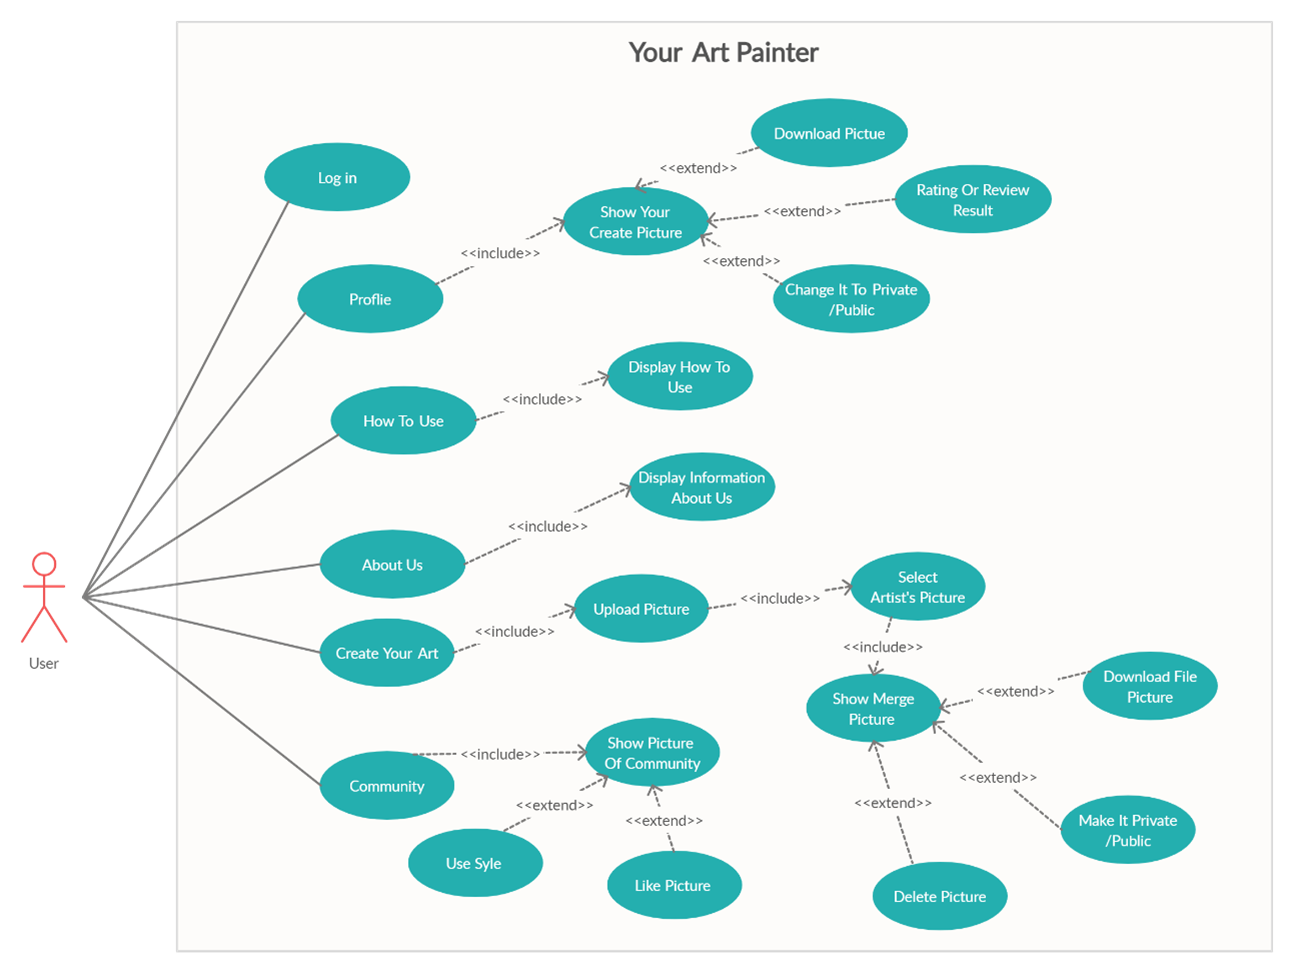
\includegraphics[width=15cm]{./image/use-case.png}
  \caption{แสดงภาพรวม Use Case Diagram}
  \label{fig:usecase}
\end{figure}

รูปที่ ~\ref{fig:usecase} แสดงความสัมพันธ์ระหว่างผู้ใช้งานกับตัวเว็บไซต์ โดยประกอบได้ด้วย 6 ระบบได้แก่


\begin{enumerate}
  \item “Log In” - ผู้ใช้สามารถลงชื่อเข้าใช้เว็บไซต์ได้ โดยใช้ email ในการเข้าสู่ระบบ
  \item “Profile” – แสดงรายละเอียดเกี่ยวกับผู้ใช้ง่าน เช่น email ที่ใช้ในการสมัคร, รูปภาพที่เคยทำการสร้างภายในเว็บไซต์ เป็นต้น
  \item “How to use” – แสดงรายละเอียดเกี่ยวกับวิธีการใช้งานเว็บไซต์
  \item “About us” – แสดงรายละเอียดเกี่ยวกับวัตถุประสงค์และผู้จัดทำเว็บไซต์ 
  \item “Create your art” - ระบบสร้างรูปภาพใหม่
  \item “Community” – ระบบชุมชนที่ซึ่งให้ผู้ใช้งานท่านอื่นมาแสดงรูปภาพที่ตนเองสร้างขึ้นมาภายในเว็บไซต์
\end{enumerate}

\newpage
\subsection{แผนภาพกิจกรรม (Activity Diagram)}
\subsubsection{ระบบลงชื่อเข้าใช้งาน}

\begin{figure}[!h]
  \centering
  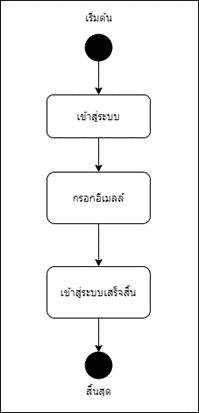
\includegraphics[width=5cm]{./image/ad-login.png}
  \caption{แสดงระบบลงชื่อเข้าใช้งาน}
  \label{fig:ad-login}
\end{figure}


\begin{table}[!h]
  \caption{ตารางอธิบายระบบลงชื่อเข้าใช้}\label{tbl:ad-login}
  \begin{tabular}{|l|l|}
  \hline
  \rowcolor[HTML]{DAE8FC} 
  \multicolumn{2}{|l|}{ตารางคำอธิบาย : ระบบการลงชื่อเข้าใช้งาน}                                                                                                                                                                                                       \\ \hline
  คำอธิบาย        & การลงชื่อเข้าใช้งาน                                                                                                                                                                                                                               \\ \hline
  จุดเริ่มต้น     & ผู้ใช้งานเข้าถึง URL ในการล็อกอิน ผ่านทางเว็บบราวเซอร์                                                                                                                                                                                            \\ \hline
  เงื่อนไขตั้งต้น & -                                                                                                                                                                                                                                                 \\ \hline
  เงื่อนไขหลังใช้ & ผู้ใช้งานจะต้องเข้าสู่ระบบ จึงจะสามารถเข้าถึงฟังก์ชั่นการทำงานต่าง ๆ                                                                                                                                                                              \\ \hline
  ขั้นตอนหลัก     & \begin{tabular}[c]{@{}l@{}}ผู้ใช้งานลงชื่อเข้าใช้โดยใช้ email ในการเข้าสู่ระบบ ตัวระบบจะทำการดึงข้อมูลจากฐานข้อมูล ถ้าตัวระบบตรวจสอบว่า email \\ ที่ผู้ใช้งานใช้เข้าสู่ระบบยังไม่มีในฐานข้อมูล ตัวระบบจะทำการสร้างบัญชีผู้ใช้ให้ใหม่\end{tabular} \\ \hline
  ขั้นตอนพิเศษ    & -                                                                                                                                                                                                                                                 \\ \hline
  \end{tabular}
  \end{table}

\newpage

\subsubsection{ระบบบัญชีผู้ใช้}

\begin{figure}[!h]
  \centering
  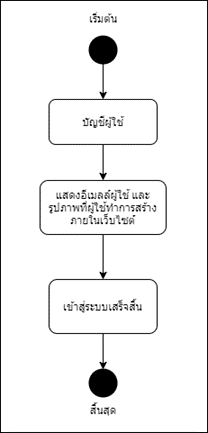
\includegraphics[width=5cm]{./image/ad-user.png}
  \caption{แสดงระบบบัญชีผู้ใช้งาน}
  \label{fig:ad-user}
\end{figure}

\begin{table}[!h]
  \caption{ตารางอธิบายระบบบัญชีผู้ใช้งาน}\label{tbl:ad-user}
  \begin{tabular}{|l|l|}
  \hline
  \rowcolor[HTML]{DAE8FC} 
  \multicolumn{2}{|l|}{ตารางคำอธิบาย : ระบบบัญชีผู้ใช้งาน}                                                                                                                                                                                                                                                                                                                     \\ \hline
  คำอธิบาย        & ระบบบัญชีผู้ใช้งาน                                                                                                                                                                                                                                                                                                                                         \\ \hline
  จุดเริ่มต้น     & ผู้ใช้กด บัญชีผู้ใช้                                                                                                                                                                                                                                                                                                                                       \\ \hline
  เงื่อนไขตั้งต้น & ผู้ใช้งานต้องทำการลงชื่อเข้าใช้โดยใช้อีเมลล์ในการเข้าใช้งาน                                                                                                                                                                                                                                                                                                \\ \hline
  เงื่อนไขหลังใช้ & ผู้ใช้งานสามารถเข้าสู่ระบบได้                                                                                                                                                                                                                                                                                                                              \\ \hline
  ขั้นตอนหลัก     & \begin{tabular}[c]{@{}l@{}}คลิก “Profile” เพื่อเข้าสู่หน้าบัญชีผู้ใช้งาน ตัวระบบจะทำการแสดงข้อมูลรายละเอียดต่าง เช่นอีเมลล์ที่\\ ใช้งาน รูปภาพที่ผู้ใช้ทำการสร้างภายในเว็บไซต์ หรือให้รูปภาพที่สร้างมานั้นแสดงในชุมชน หรือปิดการ\\ แสดงในชุมชน จำนวนยอดถูกใจแต่ละรูปภาพ ให้คะแนนความพึงพอใจกับผลลัพธ์รูปภาพหรือรายงาน\\ ผลลัพธ์ให้กับผู้พัฒนา\end{tabular} \\ \hline
  ขั้นตอนพิเศษ    & -                                                                                                                                                                                                                                                                                                                                                          \\ \hline
  \end{tabular}
\end{table}

\newpage


\subsubsection{ระบบวิธีการใช้งาน}

\begin{figure}[!h]
  \centering
  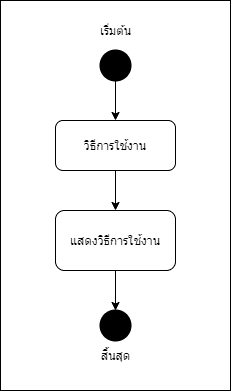
\includegraphics[width=5cm]{./image/ad-howTOuse.png}
  \caption{แสดงระบบวิธีการใช้งาน}
  \label{fig:ad-howTouse}
\end{figure}

\begin{table}[!h]
  \caption{ตารางอธิบายระบบวิธีการใช้งาน}\label{tbl:ad-howTouse}
  \begin{tabular}{|l|l|}
  \hline
  \rowcolor[HTML]{DAE8FC} 
  \multicolumn{2}{|l|}{ตารางคำอธิบาย : ระบบวิธีการใช้งาน}                                                                                                         \\ \hline
  คำอธิบาย        & ระบบวิธีการใช้งาน                                                                                                                             \\ \hline
  จุดเริ่มต้น     & ผู้ใช้กด วิธีการใช้งาน                                                                                                                        \\ \hline
  เงื่อนไขตั้งต้น & -                                                                                                                                             \\ \hline
  เงื่อนไขหลังใช้ & -                                                                                                                                             \\ \hline
  ขั้นตอนหลัก     & \begin{tabular}[c]{@{}l@{}}กด “How to use ” เพื่อเข้าสู่หน้าแสดงวิธีการใช้งานเว็บไซต์ ตัวระบบจะแสดงขั้นตอนในการ\\ ใช้งานเว็บไซต์\end{tabular} \\ \hline
  ขั้นตอนพิเศษ    & -                                                                                                                                             \\ \hline
  \end{tabular}
\end{table}

\newpage

\subsubsection{ระบบเกี่ยวกับเรา}
\begin{figure}[!h]
  \centering
  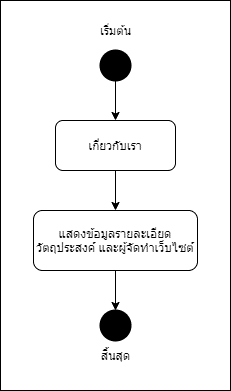
\includegraphics[width=5cm]{./image/ad-aboutUs.png}
  \caption{แสดงระบบเกี่ยวกับเรา}
  \label{fig:ad-howTouse}
\end{figure}

\begin{table}[!h]
  \caption{ตารางอธิบายระบบเกี่ยวกับเรา}\label{tbl:ad-howTouse}
  \begin{tabular}{|l|l|}
  \hline
  \rowcolor[HTML]{DAE8FC} 
  \multicolumn{2}{|l|}{ตารางคำอธิบาย : ระบบเกี่ยวกับเรา}                                                                                                                \\ \hline
  คำอธิบาย        & ระบบเกี่ยวกับเรา                                                                                                                                    \\ \hline
  จุดเริ่มต้น     & ผู้ใช้กด เกี่ยวกับเรา                                                                                                                               \\ \hline
  เงื่อนไขตั้งต้น & -                                                                                                                                                   \\ \hline
  เงื่อนไขหลังใช้ & -                                                                                                                                                   \\ \hline
  ขั้นตอนหลัก     & \begin{tabular}[c]{@{}l@{}}กด “About us” เพื่อเข้าสู่หน้าเกี่ยวกับเรา ตัวระบบจะแสดงข้อมูลรายละเอียดวัตถุประสงค์ และผู้จัดทำ\\ เว็บไซต์\end{tabular} \\ \hline
  ขั้นตอนพิเศษ    & -                                                                                                                                                   \\ \hline
  \end{tabular}
  \end{table}

\newpage

\subsubsection{ระบบสร้างรูปภาพ}
\begin{figure}[!h]
  \centering
  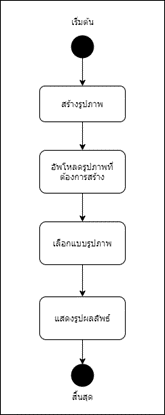
\includegraphics[width=5cm]{./image/ad-createPic.png}
  \caption{แสดงระบบเกี่ยวกับเรา}
  \label{fig:ad-createPic}
\end{figure}

\begin{table}[!h]
  \caption{ตารางอธิบายระบบสร้างรูปภาพ}\label{tbl:ad-createPic}
  \begin{tabular}{|l|l|}
  \hline
  \rowcolor[HTML]{DAE8FC} 
  \multicolumn{2}{|l|}{ตารางคำอธิบาย : ระบบสร้างรูปภาพ}                                                                                                                                                                                                                                                                                              \\ \hline
  คำอธิบาย        & การสร้างรูปภาพจากภายในเว็บไซต์                                                                                                                                                                                                                                                                                                   \\ \hline
  จุดเริ่มต้น     & ผู้ใช้กด สร้างรูปภาพ                                                                                                                                                                                                                                                                                                             \\ \hline
  เงื่อนไขตั้งต้น & -                                                                                                                                                                                                                                                                                                                                \\ \hline
  เงื่อนไขหลังใช้ & ผู้ใช้งานจะได้รับไฟล์ภาพ   ที่ผู้ใช้ทำการสร้างรูปภาพขึ้นมา                                                                                                                                                                                                                                                                       \\ \hline
  ขั้นตอนหลัก     & \begin{tabular}[c]{@{}l@{}}กด “Create your art” เพื่อเข้าสู่หน้าการสร้างรูปภาพ   จากนั้นให้ผู้ทำการอัพโหลดรูปภาพที่ต้องการให้\\ เป็น content เพื่อทำการสร้างภาพใหม่ จากนั้นเลือก style image จากภาพของศิลปิน กด submit\\ จากนั้นตัวระบบจะทำการสร้างรูปภาพใหม่ให้ผู้ใช้   โดยจะใช้เวลาประมาณ 10-15นาที ในการสร้างภาพ\end{tabular} \\ \hline
  ขั้นตอนพิเศษ    & \begin{tabular}[c]{@{}l@{}}กรณีที่ผู้ใช้สร้างภาพใหม่เป็นภาพแรกในแต่ละครั้งของการเข้าใช้ ก่อนที่ผู้ใช้จะกด submit \\ เพื่อสร้างภาพใหม่ได้นั้น ผู้ใช้จำเป็นต้องใส่อีเมลล์ เพื่อเป็นการเข้าใช้งานเว็บไซต์\end{tabular}                                                                                                              \\ \hline
  \end{tabular}
  \end{table}
\newpage

\subsubsection{ระบบชุมชน}
\begin{figure}[!h]
  \centering
  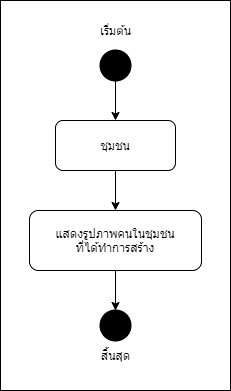
\includegraphics[width=5cm]{./image/ad-commu.png}
  \caption{แสดงระบบชุมชน}
  \label{fig:ad-commu}
\end{figure}

\begin{table}[!h]
  \caption{ตารางอธิบายระบบชุมชน}\label{tbl:ad-commu}
  \begin{tabular}{|l|l|}
  \hline
  \rowcolor[HTML]{DAE8FC} 
  \multicolumn{2}{|l|}{ตารางคำอธิบาย : ระบบชุมชน}                                                                                                                                                                                                                                                    \\ \hline
  คำอธิบาย        & ระบบชุนชนที่ให้ผู้ใช้งานเว็บไซต์แสดงผลงานให้เยี่ยมชมเว็บไซต์                                                                                                                                                                                                                     \\ \hline
  จุดเริ่มต้น     & ผู้ใช้กด ชุมชน                                                                                                                                                                                                                                                                   \\ \hline
  เงื่อนไขตั้งต้น & -                                                                                                                                                                                                                                                                                \\ \hline
  เงื่อนไขหลังใช้ & -                                                                                                                                                                                                                                                                                \\ \hline
  ขั้นตอนหลัก     & \begin{tabular}[c]{@{}l@{}}กด “Community” เพื่อเข้าสู่หน้าชุมชน ตัวระบบจะทำการแสดงผลงานการสร้างรูปภาพภายในเว็บไซต์\\ ให้ผู้เยี่ยมชม ผู้ใช้สามารถกด ถูกใจ เพื่อแสดงความชื่นชอบแก่ผลงานของผู้ใช้ท่านอื่นๆ หรือเลือกใช้ style image \\ แบบเดียวกับผู้ใช้งานท่านอื่นได้\end{tabular} \\ \hline
  ขั้นตอนพิเศษ    & -                                                                                                                                                                                                                                                                                \\ \hline
  \end{tabular}
  \end{table}

\newpage

\section{ไดอะแกรมสถาปัตยกรรมและคำอธิบาย}
\par\setlength{\parindent}{5ex}
ใช้โมเดล VGGNet ที่มีอัลกอริทึม Convolutional neural network (CNN) อยู่เบื้องหลัง โดย VGG19 เป็น pre-train ซึ่งเป็นโมเดลที่มีคน train โมเดลด้วยรูปภาพมหาศาลแล้วทำให้ไม่จำเป็นต้องมา train ใหม่เองทั้งหมด ภายใน VGGNet มีโมเดลข้างใน 2 ตัวคือ VGG16 และ VGG19

\subsection{User interface design}

\begin{figure}[!h]
  \centering
  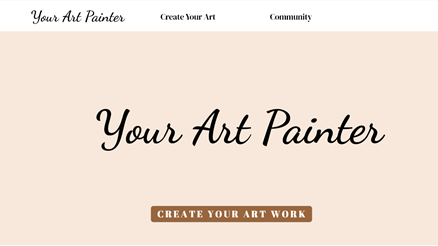
\includegraphics[width=10cm]{./image/ui1.png}
  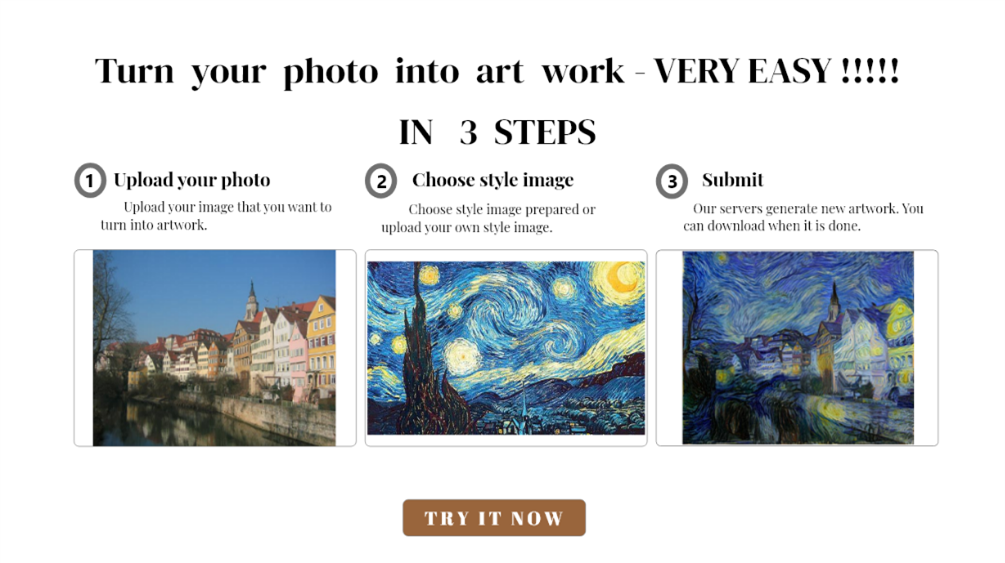
\includegraphics[width=10cm]{./image/ui1-2.png}
  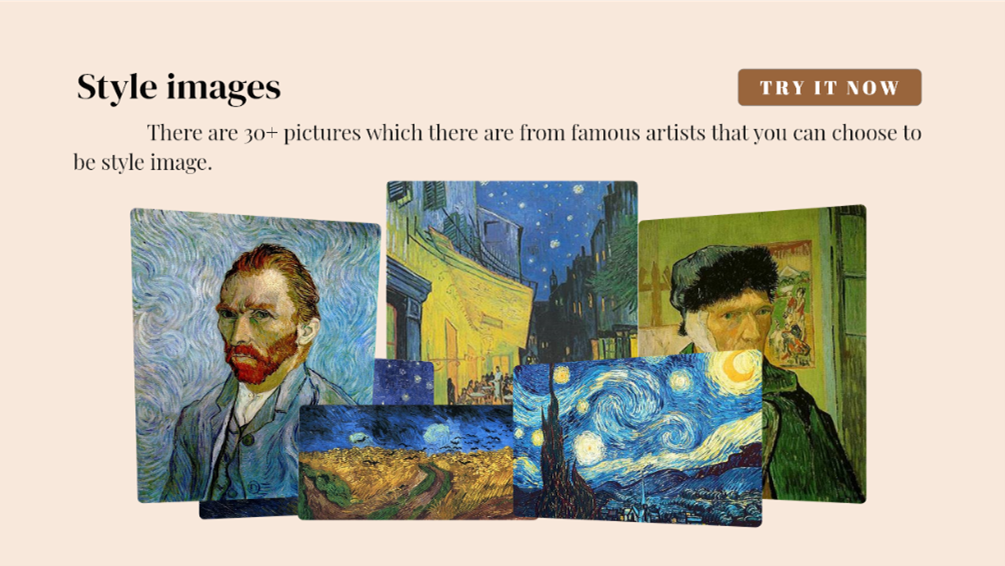
\includegraphics[width=10cm]{./image/ui1-3.png}
  \label{fig:ui}
\end{figure}

\begin{figure}[!h]
  \centering
  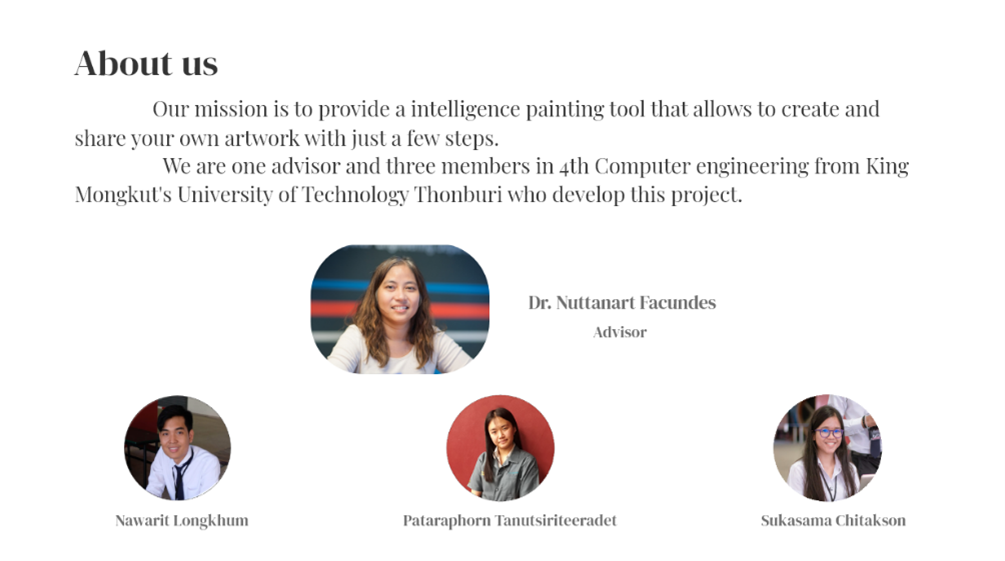
\includegraphics[width=10cm]{./image/ui1-4.png}
  \caption{แสดงหน้า Homepage}
  \label{fig:ui-1}
\end{figure}

\newpage

\par\setlength{\parindent}{5ex}
รูปที่~\ref{fig:ui-1} แสดงหน้าแรกของ web application ซึ่งเป็นหน้าที่ผู้ทุกคนจะเห็นเหมือนกันเมื่อเริ่มต้นเข้าใจ web application ของเรา โดยบทแถบเมนูของเราจะประกอบไปด้วยฟีเจอร์ create your art และ community ให้ผู้ใช้สามารถกดเข้าไปใช้งานได้ เนื้อหาที่แสดงในหน้า Homepage จะประกอบไปด้วยขั้นตอนการสร้างรูปภาพใหม่ style image และข้อมูลผู้พัฒนา web application นี้

\begin{figure}[!h]
  \centering
  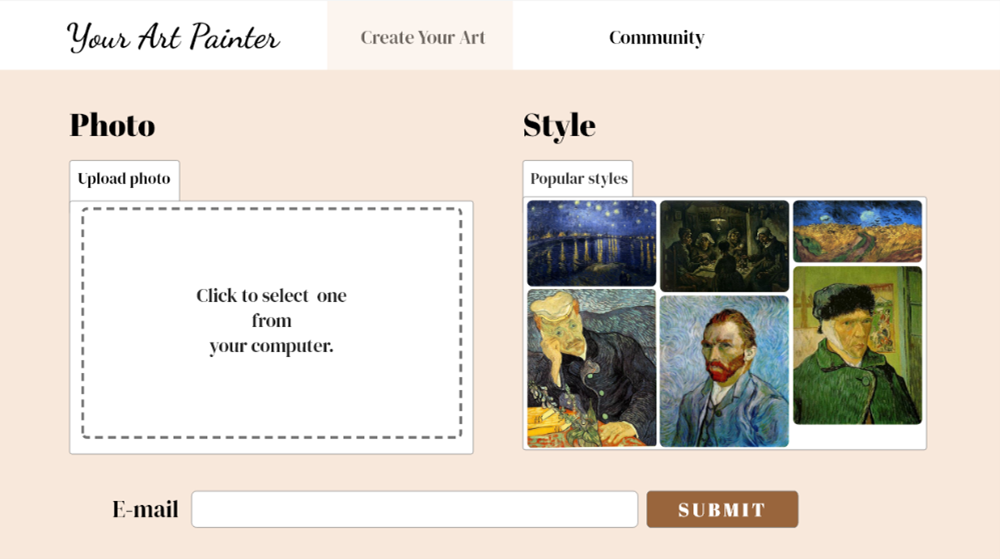
\includegraphics[width=10cm]{./image/ui-create.png}
  \caption{แสดงหน้า create your art ในขั้นตอนการเลือก content image และ style image}
  \label{fig:ui-create}
\end{figure}
\par\setlength{\parindent}{5ex}
รูปที่~\ref{fig:ui-create} เป็นหน้าที่แสดงเมื่อผู้ใช้คลิกมาใช้ฟีเจอร์ create your art ซึ่งผู้ใช้จะต้องเลือกรูปภาพที่ต้องการเป็น content image ในการสร้างภาพใหม่ (ด้านซ้าย) และเลือก style image จากภาพของศิลปิน (ด้านขวา) หากผู้ใช้สร้างภาพใหม่เป็นภาพแรกในแต่ละครั้งของการเข้าใช้ ก่อนที่ผู้ใช้จะกด submit เพื่อสร้างภาพใหม่ได้นั้น ผู้ใช้จำเป็นต้องใส่ E-mail เพื่อเป็นการ log in เข้าใช้งาน web application ก่อน หากเป็นการสร้างรูปที่ 2 เป็นต้นไป ไม่จำเป็นต้องใส่ E-mail ใหม่อีกครั้ง

\newpage
\begin{figure}[!h]
  \centering
  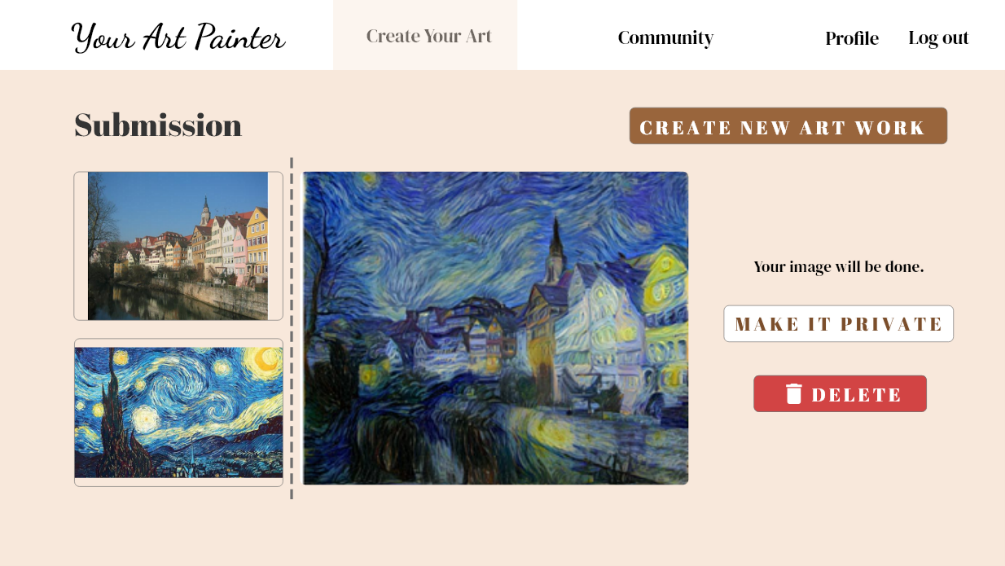
\includegraphics[width=10cm]{./image/ui-create2.png}
  \caption{แสดงหน้า create your art ในขั้นตอนการเลือก content image และ style image}
  \label{fig:ui-create2}
\end{figure}
\par\setlength{\parindent}{5ex}
รูปที่~\ref{fig:ui-create2} เป็นหน้าที่แสดงหลังจากที่ผู้ใช้กด submit เพื่อสร้างรูปใหม่แล้ว โดยหน้านี้จะแสดง content image ที่ผู้ใช้ upload มา style image ที่ผู้ใช้เลือก และภาพที่ได้หลังจากทำการประมวลผลเสร็จ หากผู้ใช้ต้องการลบภาพที่ผู้ใช้สร้างขึ้นมาก็สามารถกดปุ่ม DELETE เพื่อลบได้ หลังจากการประมวลผล ภาพที่ได้จะถูกโพสต์ไปยัง Community อัตโนมัติหากผู้ใช้ไม่ต้องการโพสต์ลงใน Community ผู้ใช้สามารกดปุ่ม MAKE IT PRIVATE ได้

\begin{figure}[!h]
  \centering
  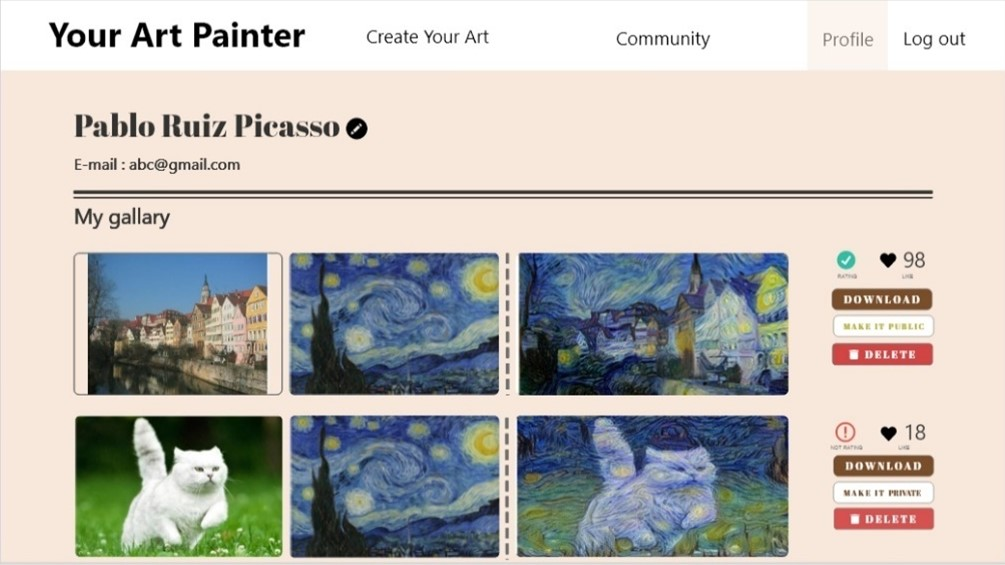
\includegraphics[width=10cm]{./image/ui-profile.jpg}
  \caption{แสดงหน้า profile}
  \label{fig:ui-profile}
\end{figure}

\par\setlength{\parindent}{5ex}
รูปที่~\ref{fig:ui-profile} แสดงหน้า profile ของผู้ใช้ โดยจะแสดง E-mail ของผู้ใช้ และรูปภาพที่ผู้ใช้ทำการสร้างขึ้น โดยประกอบไปด้วย content image, style image และรูปภาพที่ได้หลังจากการสร้างใหม่ อีกทั้งยังแสดงจำนวนคนที่กดถูกใจ ปุ่ม DOWNLOAD เพื่อให้ผู้ใช้ได้ดาวน์โหลดรูปภาพนั้น ปุ่มให้ผู้ใช้ตั้งค่าเป็นส่วนตัว (make it private หรือ make it public) สำหรับรูปภาพนี้และปุ่ม DELETE เพื่อลบรูปภาพนั้น

\newpage

\begin{figure}[!h]
  \centering
  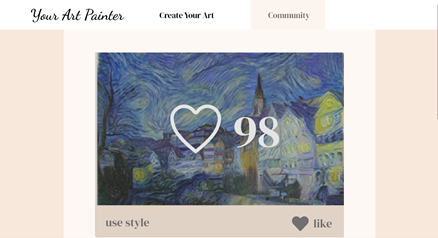
\includegraphics[width=11cm]{./image/ui-commu1.png}
  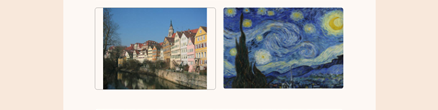
\includegraphics[width=11cm]{./image/ui-commu2.png}
  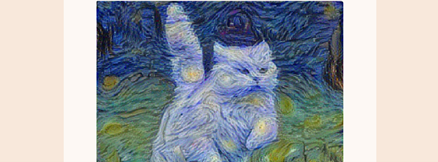
\includegraphics[width=11cm]{./image/ui-commu3.png}
  \caption{แสดงหน้า Community}
  \label{fig:ui-commu}
\end{figure}

\par\setlength{\parindent}{5ex}
รูปที่~\ref{fig:ui-commu}แสดงหน้าที่ผู้ใช้สามารถดูรูปที่มีการเผื่อแพร่ให้ผู้อื่นได้ดูของผู้ใช้ภายใน web application ได้ รวมไปถึงสามารถกดถูกใจและเลือกใช้ style นั้นได้ถ้าหากชอบจากหน้านี้

\newpage

\subsection{Database}
\begin{figure}[!h]
  \centering
  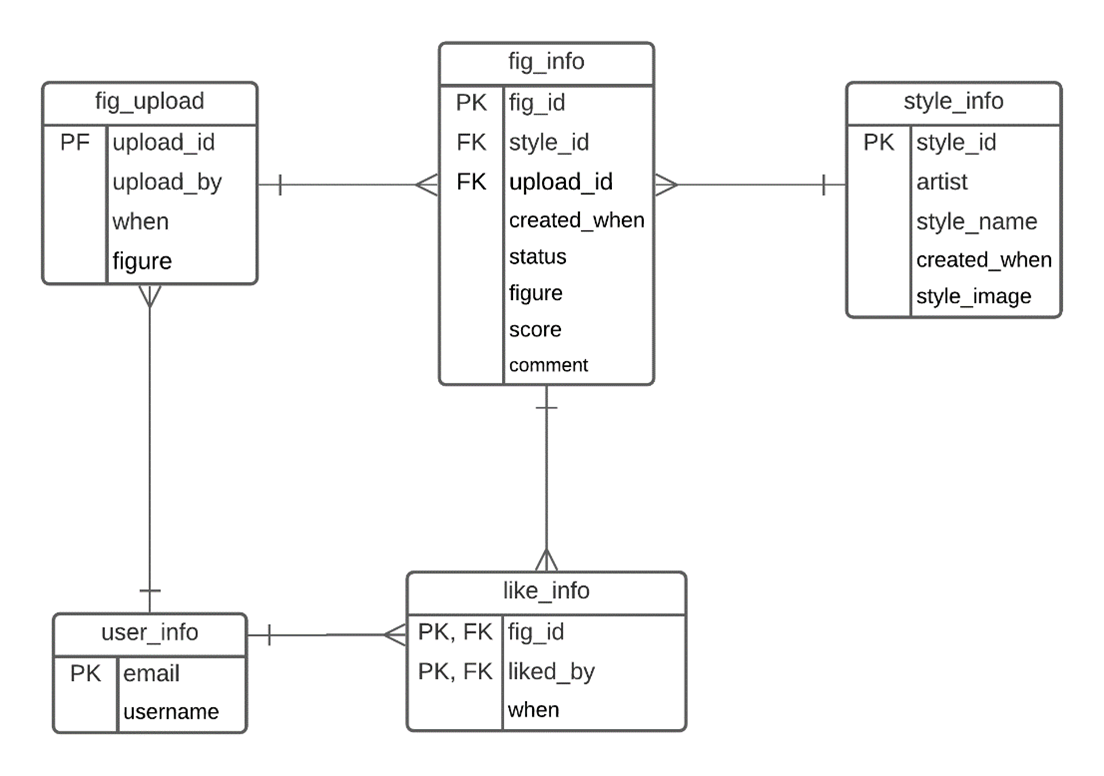
\includegraphics[width=15cm]{./image/database.png}
  \caption{แสดงหน้า Entity Relationship diagram ของ database}
  \label{fig:database}
\end{figure}
\par\setlength{\parindent}{5ex}
รูป~\ref{fig:database} แสดงภาพรวมของ database ที่ใช้ในโปรเจคนี้ ซึ่งประกอบไปด้วย 5 ตาราง ซึ่งแต่ละตารางจะมีรายละเอียดดังตารางต่อไปนี้

% Please add the following required packages to your document preamble:
% \usepackage[table,xcdraw]{xcolor}
% If you use beamer only pass "xcolor=table" option, i.e. \documentclass[xcolor=table]{beamer}
\begin{table}[!h]
  \caption{แสดงรายละเอียดของตาราง user info}\label{tbl:user_info}
  \begin{tabular}{|l|l|l|l|l|}
  \hline
  \rowcolor[HTML]{DAE8FC} 
  Entity Name & Attribute & Data Type    & Constrain & Definition                        \\ \hline
  user info   & email     & Varchar (50) & NOT NULL  & อีเมลของผู้ใช้                    \\ \hline
              & username  & Varchar (50) & NULL      & ชื่อที่แสดงใน   web   application \\ \hline
  \end{tabular}
\end{table}

\begin{table}[!h]
  \caption{แสดงรายละเอียดของตาราง fig upload}\label{tbl:fig_upload}
  \begin{tabular}{|l|l|l|l|l|}
  \hline
  \rowcolor[HTML]{DAE8FC} 
  Entity Name & Attribute  & Data Type    & Constrain & Definition                                                                                 \\ \hline
  fig\_upload & upload\_id & Integer (10) & NOT NULL  & \begin{tabular}[c]{@{}l@{}}Id ของ content image \\ ที่ผู้ใช้เลือกใช้กับภาพนี้\end{tabular} \\ \hline
              & upload\_by & Varchar (50) & NOT NULL  & อีเมลของผู้ใช้ที่ upload รูปภาพนี้                                                         \\ \hline
              & when       & TIMESTAMP    & NOT NULL  & เวลาที่ upload รูปภาพ                                                                      \\ \hline
              & figure     & GridFS       & NOT NULL  & รูปภาพ   content   ที่ผู้ใช้ upload                                                        \\ \hline
  \end{tabular}
\end{table}

\newpage

\begin{table}[!h]
  \caption{แสดงรายละเอียดของตาราง style\textunderscore info}\label{tbl:style_info1}
  \begin{tabular}{|l|l|l|l|l|}
  \hline
  \rowcolor[HTML]{DAE8FC} 
  Entity Name & Attribute     & Data Type     & Constrain & Definition                                                                                     \\ \hline
  fig\_info   & fig\_id       & Integer (10)  & NOT NULL  & Id   ของรูปภาพที่ผู้ใช้สร้างขึ้น                                                               \\ \hline
              & style\_id     & Integer (10)  & NOT NULL  & \begin{tabular}[c]{@{}l@{}}Id ของ style image ที่ใช้เลือกมา\\ ใช้กับภาพนี้\end{tabular}        \\ \hline
              & upload\_id    & Integer (10)  & NOT NULL  & \begin{tabular}[c]{@{}l@{}}Id ของ content image ที่ผู้ใช้เลือก\\ ใช้กับภาพนี้\end{tabular}     \\ \hline
              & created\_when & TIMESTAMP     & NOT NULL  & เวลาที่สร้างรูปภาพขึ้น                                                                         \\ \hline
              & status        & Boolean       & NOT NULL  & รูปนั้นแสดงผลเป็น public หรือไม่                                                               \\ \hline
              & figure        & GridFS        & NOT NULL  & รูปภาพหลังจากสร้างขึ้นใหม่                                                                     \\ \hline
              & score         & float         & NULL      & \begin{tabular}[c]{@{}l@{}}คะแนนความพึงพอใจของผู้ใช้ที่ให้\\ ต่อรูปภาพที่ประมวลผล\end{tabular} \\ \hline
              & comment       & Varchar (100) & NULL      & \begin{tabular}[c]{@{}l@{}}ความคิดเห็นต่อรูปภาพที่ประมวลผล\\ ออกมา\end{tabular}                \\ \hline
  \end{tabular}
\end{table}

\begin{table}[!h]
  \caption{แสดงรายละเอียดของตาราง style\textunderscore info}\label{tbl:style_info2}
  \begin{tabular}{|l|l|l|l|l|}
  \hline
  \rowcolor[HTML]{DAE8FC} 
  Entity Name & Attribute     & Data Type    & Constrain & Definition                                                                          \\ \hline
  style\_info & style\_id     & Integer (10) & NOT NULL  & Id ของ style image                                                                  \\ \hline
              & artist        & Varchar (50) & NOT NULL  & ชื่อศิลปินเจ้าของภาพ                                                                \\ \hline
              & style\_name   & Varchar (50) & NOT NULL  & ชื่อ style image                                                                    \\ \hline
              & created\_when & TIMESTAMP    & NOT NULL  & \begin{tabular}[c]{@{}l@{}}เวลาที่มีการ upload style image\\ นี้ขึ้นมา\end{tabular} \\ \hline
              & figure        & GridFS       & NOT NULL  & รูปภาพ content ที่ผู้ใช้ upload                                                     \\ \hline
  \end{tabular}
\end{table}

\begin{table}[!h]
  \caption{แสดงรายละเอียดของตาราง rating}\label{tbl:rating}
  \begin{tabular}{|l|l|l|l|l|}
  \hline
  \rowcolor[HTML]{DAE8FC} 
  Entity Name & Attribute  & Data Type    & Constrain & Definition                    \\ \hline
  rating      & rating\_id & Integer (10) & NOT NULL  & Id ของการให้คะแนนครั้งนั้น    \\ \hline
              & fig\_id    & Integer (10) & NOT NULL  & Id ของรูปภาพที่สร้างขึ้นมา    \\ \hline
              & rated\_by  & Varchar (50) & NOT NULL  & อีเมลของผู้ใช้ที่ให้คะแนน     \\ \hline
              & when       & TIMESTAMP    & NOT NULL  & เวลาที่มีการให้คะแนนนี้ขึ้นมา \\ \hline
              & score      & Integer      & NOT NULL  & คะแนนที่ผู้ใช้ให้             \\ \hline
  \end{tabular}
\end{table}
  
\begin{table}[!h]
  \caption{แสดงรายละเอียดของตาราง like\_info}\label{tbl:like_info}
  \begin{tabular}{|l|l|l|l|l|}
  \hline
  \rowcolor[HTML]{DAE8FC} 
  Entity Name & Attribute & Data Type    & Constrain & Definition                      \\ \hline
  Liked\_info & fig\_id   & Integer (10) & NOT NULL  & Id ของรูปภาพที่สร้างขึ้นมา      \\ \hline
              & liked\_by & Varchar (50) & NOT NULL  & อีเมลของผู้ใช้ที่ให้คะแนน       \\ \hline
              & when      & TIMESTAMP    & NOT NULL  & เวลาที่มีการให้กดถูกใจนี้ขึ้นมา \\ \hline
  \end{tabular}
\end{table}

\newpage

\subsection{Data Management}
ข้อมูลดิบที่นำมาใช้มีลักษณะเป็นรูปภาพที่อยู่ในไฟล์ PNG เป็นหลักและมีสี 3 Channel (RGB) โดยจะแยกรูปภาพออกเป็น 2 แบบ คือ
\begin{enumerate}
  \item Style image เป็นรูปภาพที่สร้างจากศิลปินที่มีชื่อเสียงโดยทางคณะผู้จัดทำเลือกรวบรวมรูปภาพที่มีลักษณะที่เด่นชัดสามารถบอกได้ว่า เป็นของศิลปินท่านไหนซึ่งเลือกศิลปินที่สนใจมา 2 ท่าน ได้แก่ อ.จักรพันธุ์ โปษยกฤษ และ อ.ชลูด นิ่มเสมอ
  \item Content image เป็นรูปภาพคนหรือสัตว์ทั่ว ๆ ไปที่ผู้ใช้ทำการอัพโหลด
\end{enumerate}

\subsection{Data structures/Class diagrams/ etc.}
\subsubsection{Software Architectural Design}

\begin{figure}[!h]
  \centering
  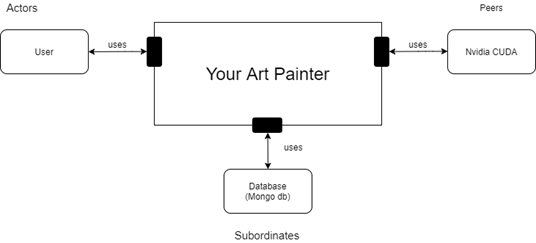
\includegraphics[width=14cm]{./image/ArchDesign.png}
  \caption{แสดงโครงสร้างพื้นฐานของระบบซอฟต์แวร์ภายในเว็บไซต์ Your Art Painter}
  \label{fig:ArchDesign}
\end{figure}
แสดงโครงสร้างพื้นฐานของระบบซอฟต์แวร์ภายในเว็บไซต์ Your Art Painter \newline
Actor
\begin{enumerate}
  \item User หรือผู้ใช้งานทั่วไป ที่เข้ามาใช้งานภายในเว็บไซต์ 
\end{enumerate}
Peers 
\begin{enumerate}
  \item Nvidia CUDA คือแพลตฟอร์มสำหรับประมวลผลแบบคู่ขนานโดยใช้ Graphic Processing Unit (GPU) ในการประมวลผล เพื่อใช้ในการประมวลผล VGG19
\end{enumerate}
Subordinates
\begin{enumerate}
  \item Mongo DB คือระบบฐานข้อมูลแบบ Nosql ใช้สำหรับเก็บข้อมูลในระบบ
\end{enumerate}

\subsection{Evaluation plans}
การประเมินผลในโครงการ แบ่งเป็น 2 ส่วนคือ ประเมินผลส่วนที่เป็นโมเดลโดยดูจากค่า loss function ที่เกิดขึ้น และเวลาให้การสร้างรูปภาพใหม่โดยเทียบกับโมเดลของ Leon A. Gatys ที่ผู้ที่ศึกษาเรื่อง Neural style transfer ใช้เป็นพื้นฐาน และอีกส่วนจะประเมินผลจากการให้บุคคลทั่วไปมาทดลองใช้งาน web application ของพวกเราเป็นจำนวน 20 คนโดยจะให้คะแนน และแสดงความคิดเห็นเกี่ยวกับผลลัพธ์ของการสร้างรูปภาพว่าผู้ใช้รู้สึกอย่างไร  

\newpage



\section{ภาคการเรียนที่ 2}
\par\setlength{\parindent}{5ex}
ในภาคการเรียนที่ 2 ทางผู้จัดทำได้ดำเนินการตามแบบแผนที่ได้จัดวางไว้โดยแบ่งแยกงานได้เป็นดังนี้

\subsection{แผนดำเนินงาน}
โดยทางผู้พัฒนาได้มีการปรับแก้ แผนการดำเนินงานในส่วนของแผนการทำงานภาคการศึกษาที่ 2 ดังนี้

\begin{table}[!h]
  \centering
  \begin{tabular}{c}
  \hfill
  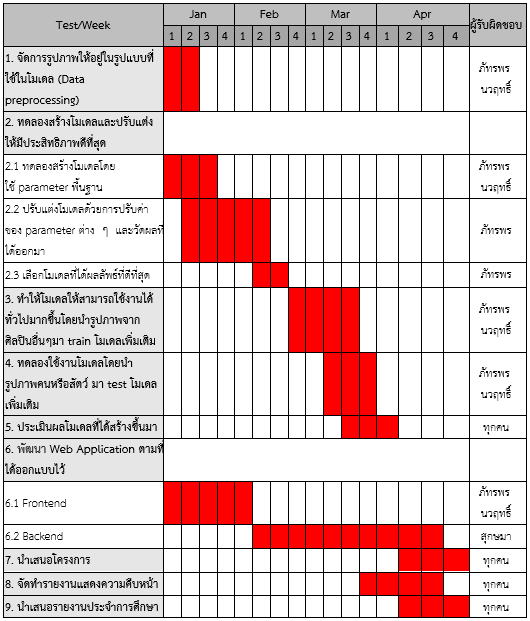
\includegraphics[width=15cm]{./image/newplan.png}
  \hfill
  \end{tabular}
\caption{ตารางแผนการทำงานภาคการศึกษาที่ 2 ใหม่\centering}
\label{tbl:newplan}
\end{table}

\newpage

\subsection{modeling}
\par\setlength{\parindent}{5ex}
ในการสร้างรูปภาพใหม่ที่มีเนื้อหาของรูปภาพเหมือนกับรูปภาพ content image ที่เป็นภาพคนหรือสัตว์ทั่วไปและมีลักษณะการวาดเหมือนกับรูปภาพ style image ของ อ.จักรพันธุ์ โปษยกฤษ และ อ.ชลูด นิ่มเสมอ ทางผู้พัฒนาได้นำวิธีการทำ Style Transfer มาใช้โดยมีวิธีการทำงานดังรูปภาพที่ ~\ref{fig:styleTransfer}

\begin{figure}[!h]
  \centering
  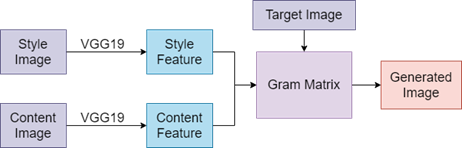
\includegraphics[width=15cm]{./image/styleTransfer.png}
  \caption{แสดงขั้นตอนการทำงานของ Style Transfer}
  \label{fig:styleTransfer}
\end{figure}

\par\setlength{\parindent}{5ex}
เนื่องจากรูปภาพ content image และ style image ทางผู้พัฒนาได้นำมาจากหลากหลายที่ทำให้ขนาดของรูปภาพมีความแตกต่างกัน จึงต้องทำ image transformation เพื่อแปลงรูปภาพให้มีขนาดที่ก่อนและใช้โมเดล VGG19 ที่มีพื้นฐานมาจาก convolutional layer ซึ่งเหมาะกับการดึงคุณลักษณะของรูปภาพ ตัวอย่างเช่น สี ลายเส้น เป็นต้นโดยดึงคุณลักษณะของรูปภาพออกมาอยู่ในรูปแบบของค่า pixel ของรูปภาพทั้ง style image และ content image จากนั้นทำการ train โดยกำหนดค่า weight ของ style feature และ content feature และใช้ gram matrix ในการจับคู่คุณลักษณะของรูปภาพที่ได้จาก style feature และ content feature เข้ากับ target image และทำการ train หลายรอบและใช้ optimizer Adam ที่มี learning rate เท่ากับ 0.03 เพื่อให้ได้ generated image ที่มีเนื้อหาของรูปภาพเหมือนกับรูปภาพ content image ที่เป็นภาพคนหรือสัตว์ทั่วไปและมีลักษณะการวาดเหมือนกับรูปภาพ style image ตามที่ต้องการ โดยทางผู้พัฒนาได้ทำการทดลองหลายรูปแบบเพื่อหาวิธีที่เหมาะสม ดังนี้
\begin{enumerate}
  \item ในขั้นตอนของการดึงคุณลักษณะของรูปภาพ โมเดล VGG19 นั้นมี pooling layer คือ max pooling ทางผู้พัฒนาได้ตั้งสมมติฐานว่า ผลลัพธ์ที่ได้ออกมาอาจมีบางจุดที่มีลักษณะเด่นเกินไปจึงทำการปรับเปลี่ยนจาก max pooling เป็น average pooling โดยกำหนดขนาดของ style image และ content image คือ 224*224 และทำการ train 5,000 รอบ
  \item จากการศึกษาจากงานวิจัย พบว่า target image ที่นำมาใช้มี 2 รูปแบบ จึงได้ทำการทดลองทั้ง 2 แบบคือ target image เป็น noise image และ target image เป็นภาพที่มาจากการคัดลอก content image ก่อนนำไปรวมกับคุณลักษณะต่าง ๆ ที่ดึงออกมาใน gram matrix โดยกำหนดขนาดของ style image และ content image คือ 224*224 ใช้โมเดล VGG19 ที่เป็น max pooling และทำการ train 5,000 รอบ
  \item ปรับเปลี่ยนขนาดของ style image เนื่องจากทางผู้พัฒนาเห็นว่า ขนาดของ style image ส่งผลต่อการดึงคุณลักษณะของรูปเพื่อทำการสร้างรูปภาพใหม่ โดยทำการปรับขนาดของรูปภาพ style image เป็น 128*128, 224*224, 512*512 และ 1024*1024 โดยกำหนดขนาดของ content image คือ 224*224 ใช้โมเดล VGG19 ที่เป็น max pooling และทำการ train 5,000 รอบ
  \item ปรับเปลี่ยนจำนวนรอบที่ใช้ในการ train เพื่อสร้างรูปภาพใหม่ โดยกำหนดเป็น 100, 500, 1,000, 5,000, 10,000, 15,000, 20,000 และ 25,000 รอบ เนื่องจากจำนวนรอบมีผลต่อลักษณะของรูปภาพที่สร้างขึ้น โดยกำหนดขนาดของ style image และ content image คือ 224*224
  \item ปรับเปลี่ยน style weight และ content weight เนื่องจากค่า weight ที่ใช้ส่งผลต่อลักษณะของรูปภาพที่สร้างขึ้นจึงได้ทำการปรับเปลี่ยนเพื่อหาค่าที่เหมาะสม
\end{enumerate}










%%%%%%%%%%%%%%%%%%%%%%%%%% บท 4 %%%%%%%%%%%%%%%%%%%%%%%%%%%%%
%%%%%%%%%%%%%%%%%%%%%%%%%%%%%%%%%%%%%%%%%%%%%%%%%%%%%%%%%%%%%%
%%%%%%%%%%%%%%%%%%%% Experiments %%%%%%%%%%%%%%%%%%%%%%%%%%%%%
%%%%%%%%%%%%%%%%%%%%%%%%%%%%%%%%%%%%%%%%%%%%%%%%%%%%%%%%%%%%%%%
\chapter{ผลการดำเนินงาน}


\section{Modeling} 
จากที่ได้ทําการทดลองตามที่ได้ออกแบบไว้ในบทที่ 3 คือ นำรูปภาพ content image ที่เป็นภาพคนหรือสัตว์และ style image ที่เป็นรูปภาพของศิลปิน อ.จักรพันธุ์ โปษยกฤษ และ อ.ชลูด นิ่มเสมอผ่านโมเดล VGG19 เพื่อดึงคุณลักษณะของรูปภาพแล้วมาผ่านการทำ gram matrix เมื่อสร้างรูปภาพใหม่ที่ผสมระหว่าง style image และ content image โดยได้ผลการทดลองจากการปรับเปลี่ยนค่าต่าง ๆ ดังนี้

\subsection{ปรับเปลี่ยนโมเดล VGG19 จาก max pooling เป็น average pooling}
 โดยกำหนดขนาดของ style image และ content image คือ 224*224 และทำการ train 5,000 รอบ พบว่ารูปภาพที่ได้จากทั้ง max pooling และ average pooling นั้นสามารถสร้างรูปภาพใหม่ที่มีการผสมระหว่าง style image และ content image และเมื่อพิจารณารูปภาพที่ได้จาก average pooling นั้นเห็นความชัดเจนของ style image ในรูปที่สร้างขึ้นมามากกว่ารูปภาพที่ได้จาก max pooling ดังรูปภาพที่ ~\ref{fig:model1}

\begin{figure}[!h]
  \centering
  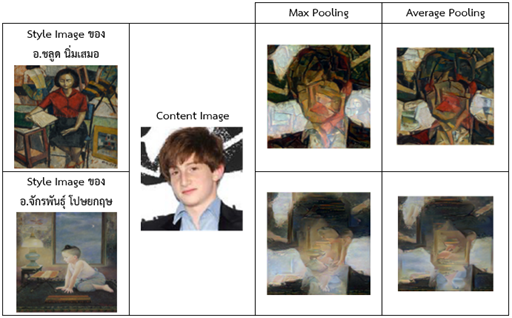
\includegraphics[width=12cm]{./image/model1.png}
  \caption{แสดงผลลัพธ์ที่ได้จากการเปลี่ยน pooling layer ใน VGG19}
  \label{fig:model1}
\end{figure}


\subsection{ทำการทดลองโดยใช้ target image เป็น noise image และ target image เป็นภาพที่มาจากการคัดลอก content image }
โดยกำหนดขนาดของ style image และ content image คือ 224*224 ใช้โมเดล VGG19 ที่เป็น max pooling และทำการ train 5,000 รอบ พบว่า target image ที่เป็น noise image นั้นไม่สามารถสร้างรูปภาพใหม่ที่มีการผสมระหว่าง style image และ content image ได้ ดังรูปภาพที่ ~\ref{fig:model2} อาจเนื่องจากการความผิดพลาดที่เกิดการวิธีการรวมคุณลักษณะของ style image และ content image ในขั้นตอนการเขียน code ก็เป็นได้

\begin{figure}[!h]
  \centering
  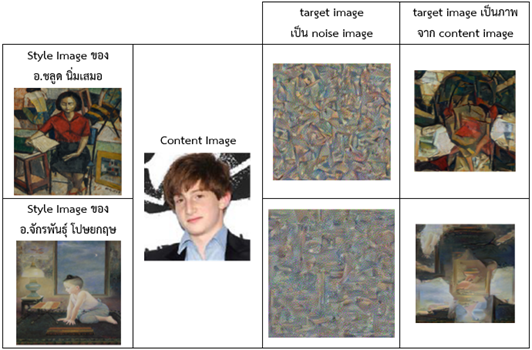
\includegraphics[width=12cm]{./image/model2.png}
  \caption{แสดงผลลัพธ์ที่เกิดจากการใช้ target image ที่แตกต่างกัน}
  \label{fig:model2}
\end{figure}

\newpage

\subsection{ปรับเปลี่ยนขนาดของ style image}
โดยได้ทำการปรับเปรี่ยน style image เป็น 128*128, 224*224, 512*512 และ 1024*1024 โดยกำหนดขนาดของ content image คือ 224*224 ใช้โมเดล VGG19 ที่เป็น max pooling และทำการ train 5,000 รอบ พบว่าการใช้ style image ขนาด 224*224 มีความเหมาะสมมากที่สุดเมื่อพิจารณาจากผลลัพธ์ที่ได้ดังรูปที่ ~\ref{fig:model3}

\begin{figure}[!h]
  \centering
  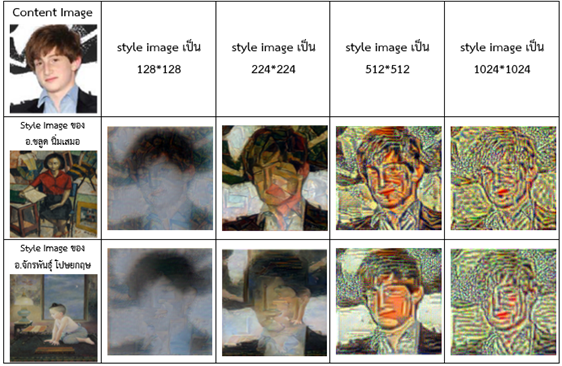
\includegraphics[width=12cm]{./image/model3.png}
  \caption{แสดงผลลัพธ์ที่เกิดจากการปรับขนาดรูปภาพ style image}
  \label{fig:model3}
\end{figure}

\pagebreak
\subsection{ปรับเปลี่ยนจำนวนรอบที่ใช้ในการ train เพื่อสร้างรูปภาพใหม่}
โดยได้ทำการปรับเปลี่ยนจำนวนรอบที่ใช้ในการ train โดยกำหนดเป็น 100, 500, 1,000, 5,000, 10,000, 15,000, 20,000 และ 25,000 รอบ โดยกำหนดขนาดของ style image และ content image คือ 224*224 พบว่า เมื่อเพิ่มจำนวนรอบ ทำให้รูปภาพใหม่ที่ได้มีการผสมระหว่าง style image และ content image ที่มากขึ้นแต่เมื่อเกิน 10,000 รอบขึ้นไป รูปภาพใหม่ที่ได้เริ่มไม่มีการเปลี่ยนแปลง ดังรูปภาพที่~\ref{fig:model4} ดังนั้นจำนวนรอบที่เหมาะสมคือ ประมาณ 5,000 รอบ

\begin{figure}[!h]
  \centering
  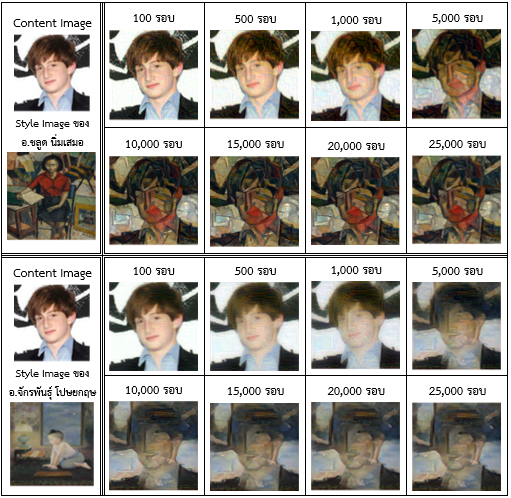
\includegraphics[width=12cm]{./image/model4.png}
  \caption{แสดงผลลัพธ์ที่เกิดจากการเพิ่มจำนวนรอบในการ train เพื่อสร้างรูปภาพใหม่}
  \label{fig:model4}
\end{figure}

\subsection{ปรับเปลี่ยน style weight และ content weight}
เนื่องจากค่า weight ที่ใช้ส่งผลต่อลักษณะของรูปภาพที่สร้างขึ้นจึงได้ทำการปรับเปลี่ยนเพื่อหาค่าที่เหมาะสม โดยกำหนดขนาดของ style image และ content image คือ 224*224 ใช้โมเดล VGG19 ที่เป็น max pooling และทำการ train 5,000 รอบ จากการทดลองพบว่า style image ที่เป็นรูปภาพของ อ.ชลูด นิ่มเสมอ ค่า style weight เท่ากับ 100 และ content weight เท่ากับ 0.01 สามารถให้รูปภาพใหม่ที่ได้มีการผสมระหว่าง style image และ content image เหมาะสมที่สุด เมื่อเปรียบเทียบกับ weight ค่าอื่น ๆ ดังรูปภาพที่~\ref{fig:model5} และ style image ที่เป็นรูปภาพของ อ.จักรพันธุ์ โปษยกฤษ ค่า style weight เท่ากับ 100 และ content weight เท่ากับ 10 สามารถให้รูปภาพใหม่ที่ได้มีการผสมระหว่าง style image และ content image เหมาะสมที่สุด ดังรูปภาพที่~\ref{fig:model6}

\begin{figure}[!h]
  \centering
  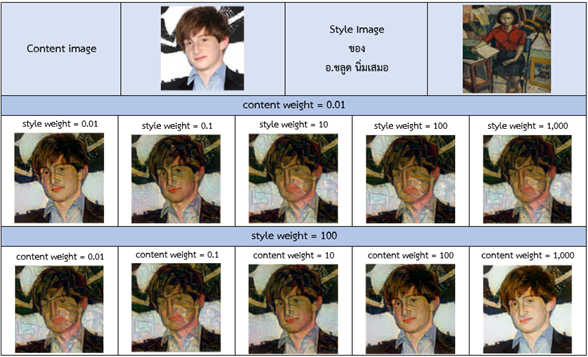
\includegraphics[width=12cm]{./image/model5.png}
  \caption{แสดงผลลัพธ์ที่เกิดจากการปรับ weight โดยใช้ style image เป็นรูปภาพของ อ.ชลูด นิ่มเสมอ}
  \label{fig:model5}
\end{figure}

\begin{figure}[!h]
  \centering
  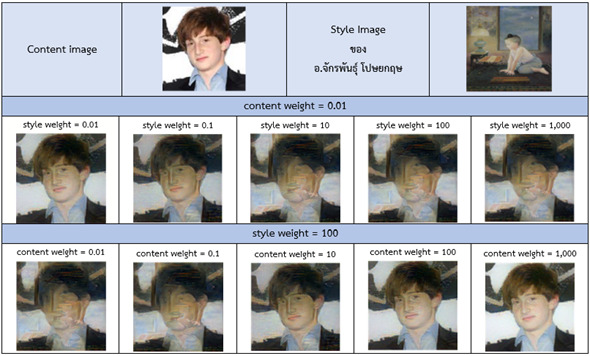
\includegraphics[width=12cm]{./image/model6.png}
  \caption{แสดงผลลัพธ์ที่เกิดจากการปรับ weight โดยใช้ style image เป็นรูปภาพของ อ.จักรพันธุ์ โปษยกฤษ}
  \label{fig:model6}
\end{figure}

\newpage
\section{WEB APPLICATION}
\subsection{User Interface }
\subsubsection{Homepage}
\begin{figure}[p]
  \centering
  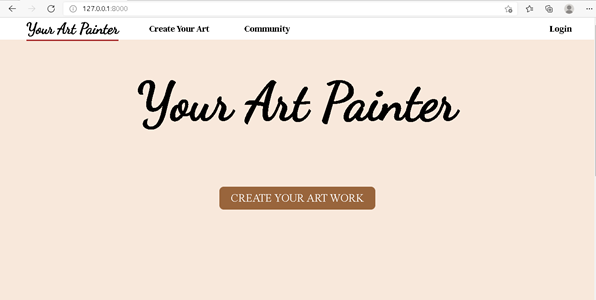
\includegraphics[width=12cm]{./image/front1.png}
  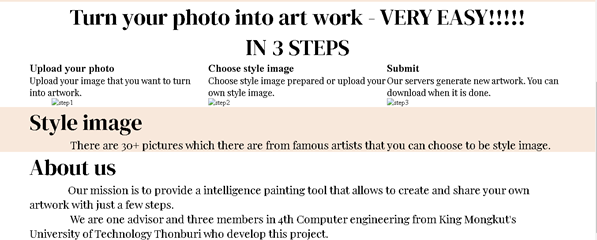
\includegraphics[width=12cm]{./image/front2.png}
  \caption{แสดงหน้า Homepage}
  \label{fig:front1-2}
\end{figure}

\subsubsection{Create your art Page}
\begin{figure}[p]
  \centering
  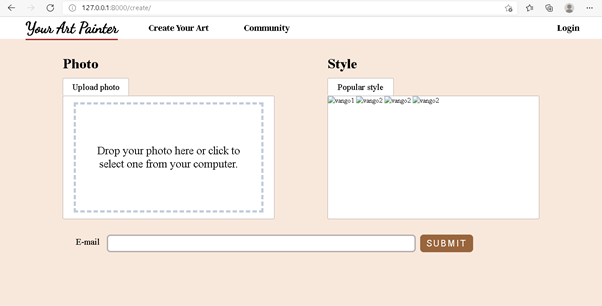
\includegraphics[width=12cm]{./image/front3.png}
  \caption{แสดงหน้า Create your art }
  \label{fig:front3}
\end{figure}

\subsubsection{Community Page}
\begin{figure}[p]
  \centering
  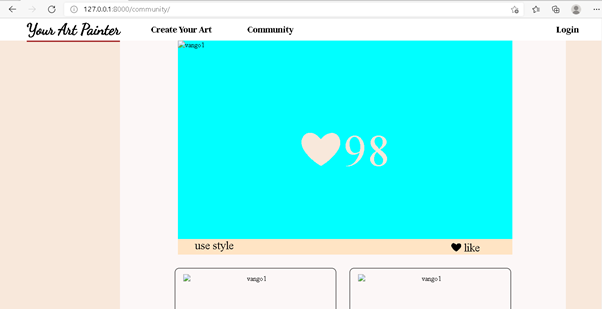
\includegraphics[width=12cm]{./image/front-commu.png}
  \caption{แสดงหน้า Community}
  \label{fig:front-commu}
\end{figure}

\subsubsection{Login Page}
\begin{figure}[p]
  \centering
  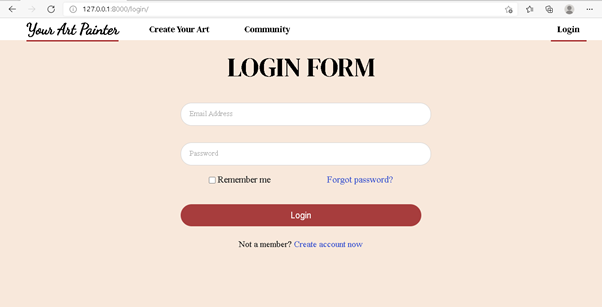
\includegraphics[width=12cm]{./image/front-login.png}
  \caption{แสดงหน้า Login}
  \label{fig:front-login}
\end{figure}

\subsubsection{Register Page}
\begin{figure}[p]
  \centering
  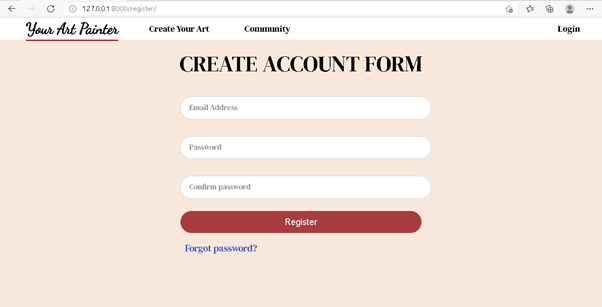
\includegraphics[width=12cm]{./image/front-regis.png}
  \caption{แสดงหน้า Register}
  \label{fig:front-regis}
\end{figure}

\newpage
\subsection{Backend และ Database}
\begin{figure}[!h]
  \centering
  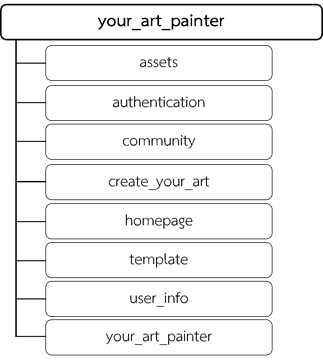
\includegraphics[width=6cm]{./image/app_module.png}
  \caption{แสดง App (module) ในส่วนของ Backend}
  \label{fig:app_module}
\end{figure}

\subsubsection{Module assets: เก็บข้อมูล static (image, css) ที่ถูกรวบรวมมาจาก directory ต่าง ๆ}
\subsubsection{Module authentication: เป็น module ที่สำหรับการ login, register}
\subsubsection{Module community: ใช้สำหรับแสดงผลภาพที่มีคนโพสต์}
\subsubsection{Module create\_your\_art: ใช้สำหรับเก็บประมวลผล Nearal style transfer}
\subsubsection{Module Homepage: ใช้สำหรับแสดงผลหน้า homepage}
\subsubsection{Module template: ใช้สำหรับเก็บ fronten ที่เป็น .html}
\subsubsection{Module user\_info:  ใช้สำหรับหน้า profile}
\subsubsection{Module your\_art\_painter: เป็น module หลักในการ setting ค่าต่าง ๆ}
\textbf{สิ่งที่ทำเสร็จ :} setting ค่าแต่ละ module ให้เชื่อมต่อกัน และconnect database ที่เป็น mongodb

\textbf{ปัญหาที่พบระหว่างทำ :} เมื่อ setting ค่าและ collectstastic ไปยัง assets กลับไม่แสดงผลอะไรเลย ทำให้ยังไม่สามารถแสดงผลรูปภาพได้




%%%%%%%%%%%%%%%%%%%%%%%%%%%%%%%%%%%%%%%%%%%%%%%%%%%%%%%%%%%%%%%
%%%%%%%%%%%%%%%%%%%% Conclusions %%%%%%%%%%%%%%%%%%%%%%%%%%%%%
%%%%%%%%%%%%%%%%%%%%%%%%%%%%%%%%%%%%%%%%%%%%%%%%%%%%%%%%%%%%%%%
\chapter{บทสรุป}

ผลสรุปของการทำโครงงาน ปัญหาที่พบระหว่างการดำเนินงานและแนวทางการแก้ไข ขอบเขต ข้อจำกัดของเครื่องมือที่พัฒนาและแนวทางการพัฒนาโครงงาน

\section{ผลการดำเนินงานในภาคการศึกษาที่ 1 (Midterm)}
ในเริ่มแรกทางผู้พัฒนาตั้งขอบเขตของโครงงานนี้คือการสร้างรูปภาพใหม่โดยการเอา Source Code ที่มีการนำ CNN ในการประมวลผลมาใช้ หลังจากนั้นทางผู้พัฒนาจะปรับปรุงการ Pre-train ขึ้นมาใหม่ให้มีความเหมาะสมมากยิ่ง โดยจะมีแบบ 3 ศิลปิน ได้แก่ 1.โกลด มอแน 2.ปาโบล รุยซ์ ปิกัสโซ และ3.วินเซนต์ แวน โก๊ะ ศิลปินละ 5 style ซึ่งหลังจากนำเสนอ Proposal presentation ได้รับข้อเสนอแนะ ว่าโครงการของผู้พัฒนาเป็นงานที่น้อยเกินไปสำหรับสมาชิก 3 คน ทางผู้พัฒนาจึงได้ทำการเปลี่ยนขอบเขตการทำโครงงานนี้ใหม่ โดยเปลี่ยนมาเป็นทำเว็บไซต์ใน การสร้างรูปภาพขึ้นมาใหม่โดยใช้ CNN ในการทำงานโดยมีแบบภาพวาด 3 ศิลปิน เช่นเดิม 

\par\setlength{\parindent}{5ex}
แต่เมื่อทางผู้พัฒนาทำการศึกษาโครงงานที่มีเนื้อหาคล้ายคลึงกับโครงการนี้ ก็มีความคิดที่จะเปลี่ยนการสร้างรูปภาพจากการ ใช้ CNN ในการสร้างรูปภาพ เปลี่ยนมาเป็นใช้  Generative Adversarial Networks หรือ GANs เหตุผลที่ทำการเลือก GANs ในการพัฒนาเพราะ GANs จะมีปัญญาประดิษฐ์ (AI) 2 ตัว ได้แก่ “Discriminator" โดยหน้าที่ของเจ้า discriminator จะทำการ classify งานที่เราต้องการให้มันทำ ยกตัวอย่างเช่น เราอยากให้มัน classify ว่ารูปภาพไหนเป็นรูปตัวเลขอาราบิก ส่วน AI ตัวที่สองจะเรียกว่า "Generator" โดยมันจะทำหน้าที่สร้างข้อมูบปลอมขึ้นมาที่มีลักษณะใกล้เคียงกับของจริงเพื่อทำการทดสอบ discriminator ยกตัวอย่างในกรณีนี้ generator จะทำการสร้างรูปตัวอักษรที่มีลักษณะคล้ายกับตัวเลขอาราบิก ซึ่งในแต่ละรอบของการทายทาง discriminator จะบอกคำตอบที่ตัวเองทายให้ generator ทราบในขณะที่ทาง generator จะให้ feedback กลับมาว่าทาง discriminator ทายถูกหรือไม่ โดยจะทำแบบนี้ต่อไปเรี่อยจน generator ไม่สามารถปรับค่าในการสร้างรูปภาพใหม่ได้ และจนที่สุดท้ายจะได้ภาพใหม่ที่เกิดจากการสร้างขึ้นมาใหม่ที่แนบเนียน สมจริงได้ดีกว่า ผลลัพธ์ของ CNN ที่รูปภาพออกมาจะมีความเป็น Filter รูปภาพเสียมากกว่าการสร้างรูปภาพ 


\par\setlength{\parindent}{5ex}
แต่เมื่อได้ทำการศึกษาทดลองดาวน์โหลด Source Code ที่ใช้หลักการ GANs ในการพัฒนา Neural Style Transfer ทางผู้พัฒนาพบปัญหาเรื่องของ library ที่ทาง Source  Code แต่ละงานวิจัยได้ทำการพัฒนาล้วนใช้ tensorflow พัฒนาเป็นหลัก ซึ่งปัญหาที่ทางผู้พัฒนาพบคือเป็น Source Code ที่มีการพัฒนา 2-3 ปีมาแล้ว ซึ่ง library tensorflow ที่ใช้ในงานวิจัยเหล่านั้นเป็นเวอร์ชั่นเก่า ทางผู้พัฒนาไม่สามารถโหลดเวอร์ชั่นที่สามารถรัน tensorflow ได้ ทั้งเวอร์ชั่น 1.13 1.14 1.15 และเวอร์ชั่น 2.0 ทางผู้พัฒนาจึงได้ประชุมกันภายในกลุ่มเพื่อหาข้อสรุปขอบเขตของโครงงานนี้ และจึงได้ข้อสรุปว่า จัดทำ web application ที่สามารถทำ Neural Style Transfer โดยจะใช้ CNN ในการพัฒนาและมีแบบสไตล์รูป 2 แบบ คือ อ.จักรพันธุ์ โปษยกฤษ และ อ.ชลูด นิ่มเสมอ โดยโมเดลที่จะนำมาใช้ทางผู้พัฒนาทำการพัฒนาขึ้นมาเอง

\section{ผลการดำเนินงานในภาคการศึกษาที่ 2 (Final) }
\par\setlength{\parindent}{5ex}
ในการดำเนินงานในภาคการศึกษาที่ 2 ทางผู้พัฒนาได้มีการปรับเปลี่ยน แผนการดำเนินงานในภาคเรียนที่ 2 ใหม่ ดังตารางที่ ~\ref{tbl:newplan} เนื่องจาก ตอนการลงมือทำจริงในส่วนของ back-end ได้มีปัญหาและอุปสรรคที่ไม่คาดคิด ทั้งในเรื่องของ การดึงรูปภาพจากฐานข้อมูลมาได้แล้ว แต่ทางเว็บแอพพลิเคชันไม่แสดงรูปภาพที่ดึงมา เป็นต้น   จึงได้ทำการปรับแก้ใหม่ ในส่วนของ front-end ของตัวเว็บไซต์สามารถพัฒนาได้ตามที่ออกแบบไว้ได้สำเร็จ 
\par\setlength{\parindent}{5ex}
ในส่วนของโมเดล ที่ใช้ในการสร้างรูปภาพใหม่ ในเว็บไซต์ของทางผู้พัฒนา  โดยเริ่มต้นทางผู้พัฒนาได้ลองใช้ soure code ที่ได้ทำเรื่อง neural style transfer แต่เป็นโมเดลที่ออกแบบมาใช้กับภาพศิลปินต่างชาติ อาทิเช่น วินเซนต์ แวน โก๊ะ หรือ ปาโบล รุยซ์ ปิกาโซ เอามาลองกับ สไตล์รูปภาพของศิลปินไทยทั้ง อ.ชลูด และอ.จักรพันธุ์ โดยเป็นการเทรนโมเดลแบบหนึ่งต่อหนึ่ง ซึ่งผลลัพธ์ที่ได้ รูปภาพใหม่ไม่ได้มีการดึงจุดเด่นของรูปภาพที่เป็นสไตล์ต้นแบบเลย หรือทำให้เกิดรูปภาพใหม่ที่ผิดแปลกไป ทางผู้พัฒนาจึงได้ทำการทดลองเพื่อหาข้อสรุปที่จะนำมาใช้กับสไตล์รูปภาพของอาจารย์ทั้ง 2 ท่าน โดยจากการทดลองที่ทางผู้พัฒนาได้ทดลองทำ สรุปได้ว่า โมเดล VGG19 ที่ใช้ดึงคุณลักษณะของรูปภาพควรใช้ max pooling ใน pooling layer ขนาดของรูปภาพ style image และ content image คือ 224*224 และ target image ควรเป็นรูปภาพที่คัดลอกมาจาก content image โดยใช้การ train เพื่อสร้างรูปภาพใหม่ที่ผสมระหว่าง style image และ content image จำนวน 5,000 รอบ โดย style image ของ อ.ชลูด นิ่มเสมอใช้ style weight เท่ากับ 100 และ content weight เท่ากับ 0.01 ส่วน style image ของ อ.จักรพันธุ์ โปษยกฤษใช้  style weight เท่ากับ 100 และ content weight เท่ากับ 10


%\section{ข้อจำกัดและข้อเสนอแนะ}
%ข้อจำกัดของโครงงาน What could be done in the future to make your projects better.






%%%%%%%%%%%%%%%%%%%%%%%%%%%%%%%%%%%%%%%%%%%%%%%%%%%%%%%%%%%%%%%
%%%%%%%%%%%%%%%%%%%% Bibliography %%%%%%%%%%%%%%%%%%%%%%%%%%%%%
%%%%%%%%%%%%%%%%%%%%%%%%%%%%%%%%%%%%%%%%%%%%%%%%%%%%%%%%%%%%%%%

%%%% Comment this in your report to show only references you have
%%%% cited. Otherwise, all the references below will be shown.
%\nocite{*}
%% Use the kmutt.bst for bibtex bibliography style 
%% You must have cpe.bib and string.bib in your current directory.
%% You may go to file .bbl to manually edit the bib items.
\bibliographystyle{kmutt}
\bibliography{string,cpe}

%%%%%%%%%%%%%%%%%%%%%%%%%%%%%%%%%%%%%%%%%%%%%%%%%%%%%%%%%%%%%%%
%%%%%%%%%%%%%%%%%%%%%%%% Appendix %%%%%%%%%%%%%%%%%%%%%%%%%%%%%
%%%%%%%%%%%%%%%%%%%%%%%%%%%%%%%%%%%%%%%%%%%%%%%%%%%%%%%%%%%%%%%
\appendix{ชื่อภาคผนวกที่ 1}
\noindent{\large\bf ใส่หัวข้อตามความเหมาะสม} \\

This is where you put hardware circuit diagrams, detailed experimental data in tables or source codes, etc.. \\ \bigskip



This appendix describes two static allocation methods for fGn (or fBm)
traffic. Here, $\lambda$ and $C$ are respectively the traffic arrival
rate and the service rate per dimensionless time step. Their unit are
converted to a physical time unit by multiplying the step size
$\Delta$. For a fBm self-similar traffic source,
%Norros~\cite{norros95} provides its EB as
\begin{equation}\label{eq:norros}
  C = \lambda + (\kappa(H)\sqrt{-2\ln\epsilon})^{1/H}a^{1/(2H)}x^{-(1-H)/H}\lambda^{1/(2H)}
\end{equation}
where $\kappa(H) = H^H(1-H)^{(1-H)}$. Simplicity in the calculation is
the attractive feature of (\ref{eq:norros}).

The MVA technique developed in~\cite{kim01} so far provides the most
accurate estimation of the loss probability compared to previous
bandwidth allocation techniques according to simulation results.
Consider a discrete-time queueing system with constant service rate
$C$ and input process $\lambda_n$ with $\mathbb{E}\{\lambda_n\} =
\lambda$ and $\mathrm{Var}\{\lambda_n\} = \sigma^2$.  Define $X_n \equiv
\sum_{k=1}^n \lambda_k - Cn$.  The loss probability due to the MVA
approach is given by
\begin{equation}\label{eq:loss_mva}
  \varepsilon \approx \alpha e^{-m_x/2}
\end{equation}
where
\begin{equation}\label{eq:mx}
m_x = \min_{n \geq 0} \frac{((C-\lambda)n + B)^2}{\mathrm{Var}\{X_n\}} =
\frac{((C-\lambda)n^\ast + B)^2}{\mathrm{Var}\{X_{n^{\ast}}\}}
\end{equation} 
and 
\begin{equation}\label{eq:alpha}
  \alpha =
  \frac{1}{\lambda\sqrt{2\pi\sigma^2}}\exp\left(\frac{(C-\lambda)^2}{2\sigma^2}\right)
  \int_C^\infty (r-C)\exp\left(\frac{(r-\lambda)^2}{2\sigma^2}\right)\, dr
\end{equation}
For a given $\varepsilon$, we numerically solve for $C$ that satisfies
(\ref{eq:loss_mva}). Any search algorithm can be used to do the task.
Here, the bisection method is used.  

Next, we show how $\mathrm{Var}\{X_n\}$ can be determined.  Let
$C_{\lambda}(l)$ be the autocovariance function of $\lambda_n$.  The
MVA technique basically approximates the input process $\lambda_n$
with a Gaussian process, which allows $\mathrm{Var}\{X_n\}$ to be
represented by the autocovariance function.  In particular, the
variance of $X_n$ can be expressed in terms of $C_{\lambda}(l)$ as
\begin{equation}
  \mathrm{Var}\{X_n\} = nC_{\lambda}(0) + 2\sum_{l=1}^{n-1} (n-l)C_{\lambda}(l)
\end{equation} 
Therefore, $C_{\lambda}(l)$ must be known in the MVA technique, either
by assuming specific traffic models or by off-line analysis in case of
traces.  In most practical situations, $C_{\lambda}(l)$ will not be
known in advance, and an on-line measurement algorithm developed
in~\cite{eun01} is required to jointly determine both $n^\ast$ and
$m_x$. For fGn traffic, $\mathrm{Var}\{X_n\}$ is equal to $\sigma^2
n^{2H}$, where $\sigma^2 = \mathrm{Var}\{\lambda_n\}$, and we can find
the $n^\ast$ that minimizes (\ref{eq:mx}) directly. Although $\lambda$
can be easily measured, it is not the case for $\sigma^2$ and $H$.
Consequently, the MVA technique suffers from the need of prior
knowledge traffic parameters.


%%%%%%%%%%%%%%%%%%%%%%%%%%%%%%%%%%%%%%%%%%%%%%%%%%%%%%%%%%
%%%%%%%%%%%%%%% The 2nd appendix %%%%%%%%%%%%%%%%%%%%%%%%%%
%%%%%%%%%%%%%%%%%%%%%%%%%%%%%%%%%%%%%%%%%%%%%%%%%%%%%%%%%%
\appendix{ชื่อภาคผนวกที่ 2}
\noindent{\large\bf ใส่หัวข้อตามความเหมาะสม} \\

Next, we show how $\mathrm{Var}\{X_n\}$ can be determined.  Let
$C_{\lambda}(l)$ be the autocovariance function of $\lambda_n$.  The
MVA technique basically approximates the input process $\lambda_n$
with a Gaussian process, which allows $\mathrm{Var}\{X_n\}$ to be
represented by the autocovariance function.  In particular, the
variance of $X_n$ can be expressed in terms of $C_{\lambda}(l)$ as
\begin{equation}
  \mathrm{Var}\{X_n\} = nC_{\lambda}(0) + 2\sum_{l=1}^{n-1} (n-l)C_{\lambda}(l)
\end{equation} 

\noindent{\large\bf Add more topic as you need} \\

Therefore, $C_{\lambda}(l)$ must be known in the MVA technique, either
by assuming specific traffic models or by off-line analysis in case of
traces.  In most practical situations, $C_{\lambda}(l)$ will not be
known in advance, and an on-line measurement algorithm developed
in~\cite{eun01} is required to jointly determine both $n^\ast$ and
$m_x$. For fGn traffic, $\mathrm{Var}\{X_n\}$ is equal to $\sigma^2
n^{2H}$, where $\sigma^2 = \mathrm{Var}\{\lambda_n\}$, and we can find
the $n^\ast$ that minimizes (\ref{eq:mx}) directly. Although $\lambda$
can be easily measured, it is not the case for $\sigma^2$ and $H$.
Consequently, the MVA technique suffers from the need of prior
knowledge traffic parameters. 





\end{document}
